\documentclass[]{article}
\usepackage{caption,subcaption,graphicx,float,url,amsmath,amssymb,tocloft}
\usepackage[hidelinks]{hyperref}
\usepackage[toc,acronym,nonumberlist]{glossaries}
\setacronymstyle{long-short}
\usepackage{glossaries-extra}
\graphicspath{{figs/}} 
\setlength{\cftsubsecindent}{0em}
\setlength{\cftsecnumwidth}{3em}
\setlength{\cftsubsecnumwidth}{3em}
\DeclareUnicodeCharacter{2192}{~}
\newcommand\numberthis{\addtocounter{equation}{1}\tag{\theequation}}

%opening
\title{
	Notes from Origins of Life\\
	Week 3: Chemical Commonalities
}

\author{Simon Crase (compiler)\\simon@greenweaves.nz}

\makeglossaries

\loadglsentries{glossary-entries}

\renewcommand{\thesection}{3.\arabic{section}}
\renewcommand{\glstextformat}[1]{\textbf{\em #1}}

\begin{document}

\maketitle

\begin{abstract}
 	These are my notes from the $3^{rd}$ week of the Santa Fe Institute Origins of Life Course\cite{sfi2020}. The course aims to push the field of Origins of Life research forward by bringing new and synthetic thinking to the question of how life emerged from an abiotic world.\\
  	The content and images contained herein are the intellectual property of the Santa Fe Institute, with the exception of any errors in transcription, which are my own.
  	These notes are distributed in the hope that they will be useful,
  	but without any warranty, and without even the implied warranty of
  	merchantability or fitness for a particular purpose. All feedback is welcome,
  	but I don't necessarily undertake to do anything with it.
\end{abstract}

\setcounter{tocdepth}{2}
\tableofcontents

\listoffigures
\listoftables

\section{Introduction}

This week is a more detailed look at biochemistry:\begin{itemize}
	\item  biological information encoded in chemistry;
	\item the chemical processes that drive organization; and
	\item  how life extracts energy from its environment.
\end{itemize}

\section[DNA as Information]{DNA as Information--Michael Lachmann}

\subsection{DNA Modification}

\begin{figure}[H]
	\begin{center}
		\caption[DNA, pairing G/C, A/T.]{DNA, pairing G/C, A/T. Mutation rate $10^{-10}$ errors per rep.base. }\label{fig:DNA}
		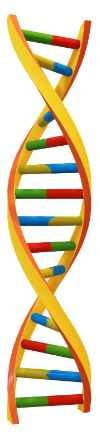
\includegraphics[width=0.1\textwidth]{DNA}
	\end{center}
\end{figure}
We kind of imagine that
somehow evolution met this magic
molecule that has all these properties
and that's how life emerged,
or that's how we got \gls{gls:DNA} -
just from the properties of the \gls{gls:DNA}.
And, in these two lectures,
I want to show you
that this is not such a right -
a correct - view,
and \gls{gls:DNA} is much more noisy
than we think
and the pairing and their bases
are much more noisy than that.

\gls{gls:DNA} has a mutation rate
of ten to the minus ten errors
per replication per base,
which is a really amazingly low rate,
and I will go a bit into
how we get such a low rate
in the next lecture.

In this lecture, I want to talk about
the bases,
and for this I need to go a bit into
the structure of nucleotides.


\begin{figure}[H]
	\caption[The 4 Nucleotides in \gls{gls:DNA}]{The 4 Nucleotides in \gls{gls:DNA}--two \glspl{gls:purine} and two \glspl{gls:pyrimidine}.}\label{fig:Nucleotides} 
	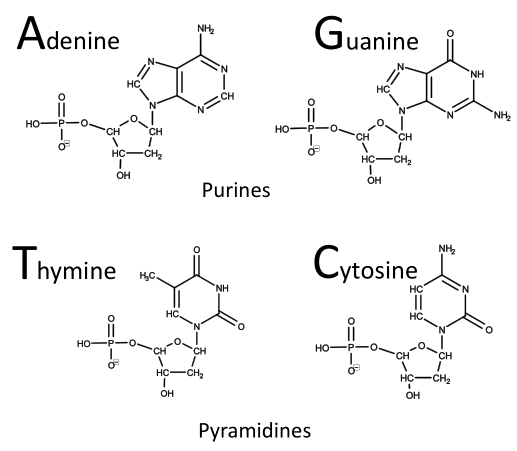
\includegraphics[width=0.9\textwidth]{Nucleotides}
\end{figure}

Let's have a closer look at one base, adenine--Figure \ref{fig:NucleotideAdenine}.
\begin{figure}[H]
	\caption[A closer look at one Nucleotide, Adenine]{A closer look at one Nucleotide, Adenine. In this lecture we won't be very concerned with the backbone.}\label{fig:NucleotideAdenine} 
	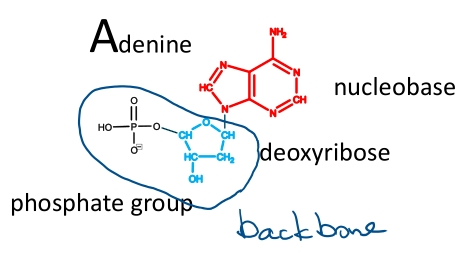
\includegraphics[width=0.9\textwidth]{NucleotideAdenine}
\end{figure}

Figure \ref{fig:NucleotideDNARNA} depicts Adenine in \gls{gls:RNA}. It shows the only \emph{chemical} difference between \gls{gls:DNA} and \gls{gls:RNA}: the extra OH group in \gls{gls:RNA}, which makes the molecule more active. \gls{gls:DNA} is more stable.
\begin{figure}[H]
	\caption[Chemical difference between DNA and RNA is the extra oxygen]{The only chemical difference between \gls{gls:DNA} and \gls{gls:RNA} is the extra oxygen in \gls{gls:RNA}. It causes \gls{gls:RNA} to be more active then \gls{gls:DNA}.}\label{fig:NucleotideDNARNA} 
	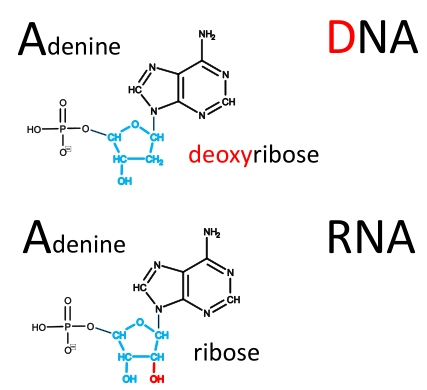
\includegraphics[width=0.9\textwidth]{NucleotideDNARNA}
\end{figure}

RNA uses Uracil instead of Thymine--Figure \ref{fig:NucleotideDNARNAThymineUracil}. Note that Thymine is Uracil with an extra methyl group, hence the alternative name $5-methyluracil$. The $5$ comes from the numbering of carbon atoms--see \ref{fig:NucleotidesCounting}
	
\begin{figure}[H]
	\caption{RNA uses Uracil instead of Thymine.} \label{fig:NucleotideDNARNAThymineUracil} 
	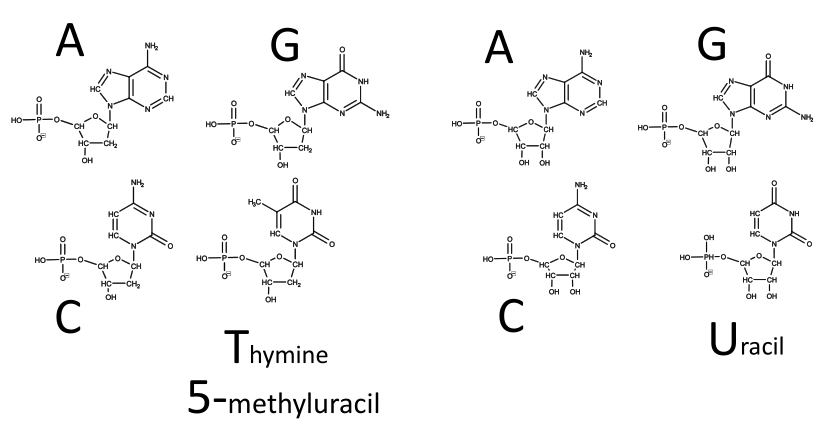
\includegraphics[width=0.9\textwidth]{NucleotideDNARNAThymineUracil}
\end{figure}

Figure \ref{fig:NucleotidesCounting} shows the way atoms are numbered in purines and pyrimidines.\begin{itemize}
	\item The counting on thymine and the other pyrimidines is very simple.
	It starts from the nitrogen that's closest to the ribose--connects to the ribose--
	and goes towards the other nitrogen, in this case counterclockwise --
	simply one, two, three, four, five, six around the ring.
	\item The counting on the purines is a bit more complicated.
	In this case, you start from the nitrogen that's furthest away from the ribose 	and count again towards the other nitrogen around the ring.
	And, when you finish the first ring -one, two, three, four, five, six - you go in the other ring... 	again to the nitrogen 	that furthest away from the ribose - 	seven, eight, nine - towards the nitrogen that's connected to the ribose.
	So, we see that thymine is a modified uracil--5-methyluracil.
\end{itemize}
\begin{figure}[H]
	\caption{Numbering of carbon atoms in purines and pyrimidines. }\label{fig:NucleotidesCounting} 
	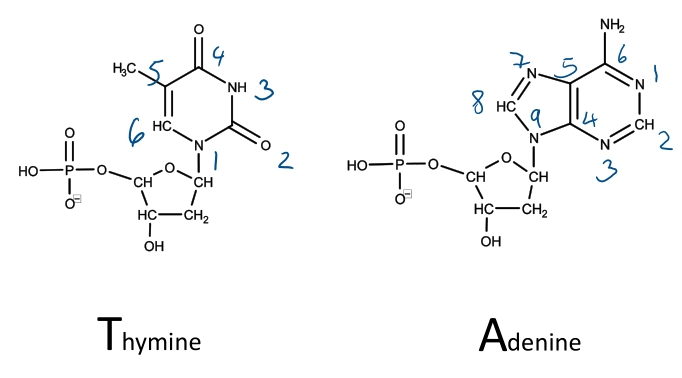
\includegraphics[width=0.9\textwidth]{NucleotidesCounting}
\end{figure}

There are many modified nucleobases.
In Figure \ref{fig:ModifiedBases}, I just listed twelve. So, here we have the five
that we know already - the four on the DNA and uracil.
In addition, I listed a couple more modified bases that you can see - one is xanthine - and several others.

\begin{figure}[H]
	\caption{A selection of 12 modified bases}\label{fig:ModifiedBases} 
	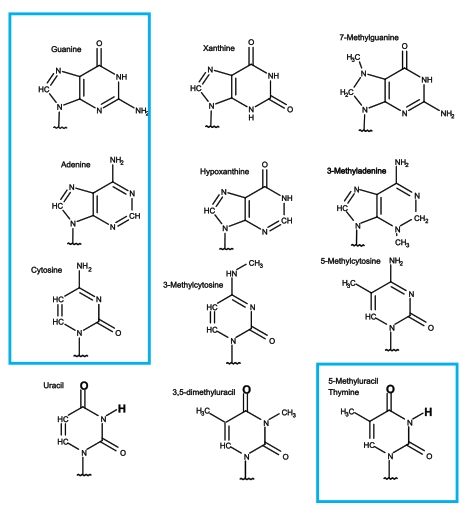
\includegraphics[width=0.9\textwidth]{ModifiedBases}
\end{figure}


There is actually a database online
that lists
all the known DNA modifications
that have been observed
actually in nature.
Figure \ref{fig:ModifiedDNA_Nucleobases} includes 44 modified nucleobases
that actually have been observed
on DNA in nature.
In addition, there is the few gray ones
that have been produced artificially.

\begin{figure}[H]
	\caption[Modified DNA nucleobases]{Modified DNA nucleobases \cite{sood2019dnamod},\cite{sood2019dnamod_website}} \label{fig:ModifiedDNA_Nucleobases} 
	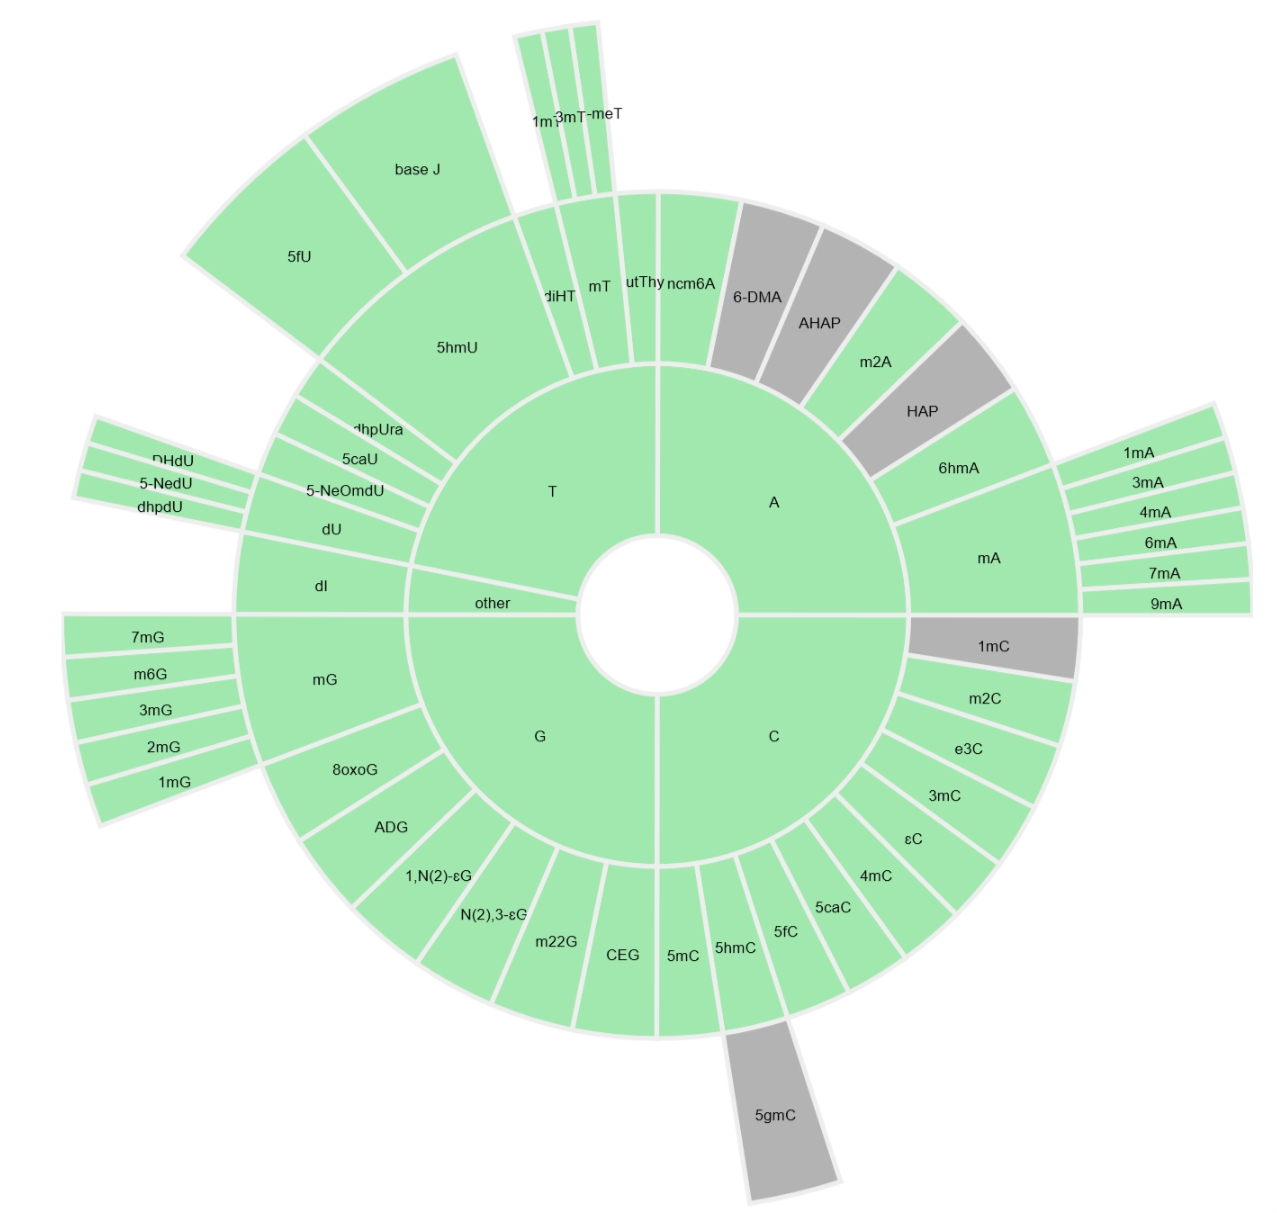
\includegraphics[width=0.9\textwidth]{ModifiedDNA_Nucleobases}
\end{figure}

The are a couple of bacteriophages, PBS1 and PBS2, that contain Uracil instead of thymine in their DNA\cite{hemphill1975bacteriophages}. Either the thymine has been replaced, or these phages are more primitive, and never used thymine.

When people talk about \gls{gls:methylation} of DNA, they usually mean 5-methylcytosine, Figure \ref{fig:5methylcytosine}, even though there are many other ways to do it
\begin{figure}[H]
	\caption{5-methylcytosine } \label{fig:5methylcytosine} 
	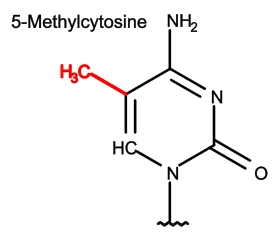
\includegraphics[width=0.9\textwidth]{5-methylcytosine}
\end{figure}

\Gls{gls:methylation} tends to occur when C is followed by G--known as \gls{gls:CpG}. The methylated versions are replicated as unmethylated C, but there is an enzyme, \gls{gls:DNAmethyltransferase}, which performs methylation, as shown in Figure \ref{fig:5-methylcytosine-in-action}. This can carry epigenetic changes across cell divisions, and sometimes across generations. This is important as it means that a liver cell can "remember" that it came from a liver cell.
\begin{figure}[H]
	\caption{Methylation tends to occur when C is followed by G and vice versa} \label{fig:5-methylcytosine-in-action} 
	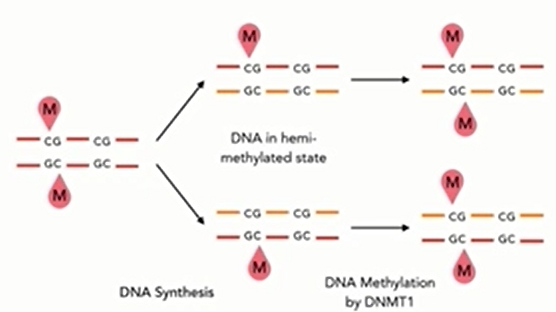
\includegraphics[width=0.9\textwidth]{5-methylcytosine-in-action}
\end{figure}

6-Methyladenine is also important--Figure \ref{fig:6-Methyladenine}-- in bacteria, where it carries information regarding the old strand versus the new. The methylation isn't very fast, so it can distinguish old from new. Section \ref{section:DNAasInfo2} shows how this is useful for repair.

\begin{figure}[H]
	\caption{6-Methyladenine is also important (palindromic sequence)} \label{fig:6-Methyladenine} 
	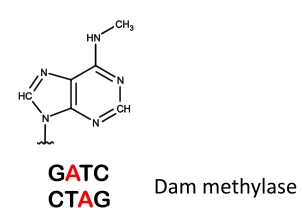
\includegraphics[width=0.9\textwidth]{6-Methyladenine}
\end{figure}

The values in Figure \ref{fig:ModifiedRNAdatabase} have been taken from the Modified RNA database \cite{agriss2019RNA}.

\begin{figure}[H]
	\caption{Modified RNA database} \label{fig:ModifiedRNAdatabase} 
	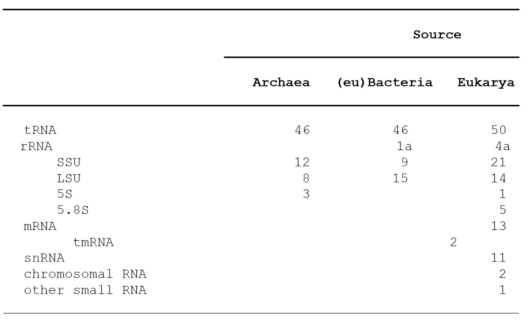
\includegraphics[width=0.9\textwidth]{ModifiedRNAdatabase}
\end{figure}

\textbf{Summary}

\begin{itemize}
	\item There are 44 known DNA modifications
	\item There are 112 known RNA modifications
	\item Many of these modifications on the DNA
	survive replication. So, the polymerase can go across them
	with no problem.
	\item Some are even replicated
	with additional enzymes.
	\item Some modifications are functional:\begin{itemize}
		\item 5-methylcytosine (5mC)
		\item N6-methadenine (6mA)
		\item 5-hydroxymethylcytosine (5hmC)
		\item Some functional in RNA
		\item It is likely there are more, since this is a fairly new field.
	\end{itemize}
	\item How are they generated?
	\begin{itemize}
		\item Enzyme activity
		\item Damage
		\item Misincorporation
	\end{itemize}
\end{itemize}

Where did the modifications come from? They could be fairly new, and we use them in various ways; or maybe they tell us something about the origin of DNA. Maybe there are many enzymes left over from before we had sophisticated machinery for DNA replication.

\subsection{DNA base pairing}\label{section:DNAasInfo2}

In this lecture we discuss how pairing is controlled, and how the error rates is kept so low--$10^{-10}$ per (replication*base pair). Usually base pairs are presented as in Figure \ref{fig:BasePairsML}: A only fits T, and C only fits G. Figure \ref{fig:BasePairsML_hydrogen_bonds} shows how this is implemented with hydrogen bonds.
\begin{figure}[H]
		\caption{Base Pairs}
		\begin{subfigure}[t]{0.4\textwidth}
			\caption{A only fits T; C only fits G.}\label{fig:BasePairsML}
			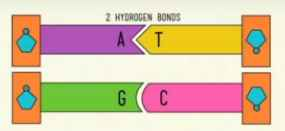
\includegraphics[width=\textwidth]{BasePairsML}
		\end{subfigure}
		\begin{subfigure}[t]{0.55\textwidth}
			\caption{Figure \ref{fig:BasePairsML} with hydrogen bonds}\label{fig:BasePairsML_hydrogen_bonds}
			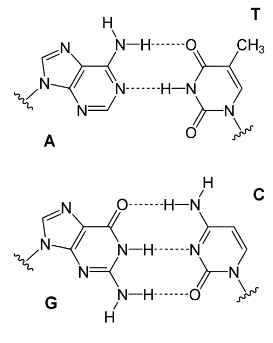
\includegraphics[width=\textwidth]{BasePairsML_hydrogen_bonds}
		\end{subfigure}
\end{figure}

\subsubsection{DNA polymerase}
I will just talk about DNA polymerase,
which allows DNA replication
to achieve a very low rate.
Let's look at the reaction.
So, usually in any reaction
we have reactants and products.
And, we're interested in the rate of going
from reactants to products...
or both rates going forward
and backward.
Rate going forward usually is calculated
by the \gls{gls:arrheniusequation},
which gives us $e^{-\frac{E_A}{kT}}$--Figure \ref{fig:ArrheniusEquation}.
So, the higher the activation energy,
the slower the reaction will be.

\begin{figure}[H]
	\caption{The rate of going from reactants to products}
	\begin{subfigure}[t]{0.3\textwidth}
		\caption{Rate going forward is calculated using the Arrhenius Equation}\label{fig:ArrheniusEquation}
		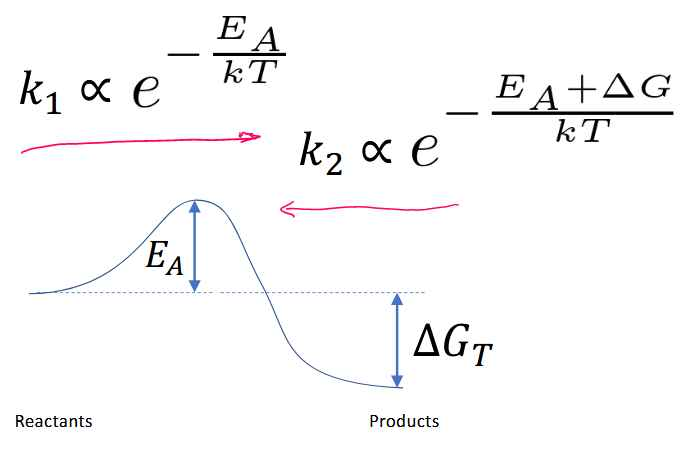
\includegraphics[width=\textwidth]{ArrheniusEquation}
	\end{subfigure}
	\;
	\begin{subfigure}[t]{0.3\textwidth}
		\caption{If reactants and products
			have different free energy,
			then there's also $\Delta G$}\label{fig:ArrheniusEquation2}
		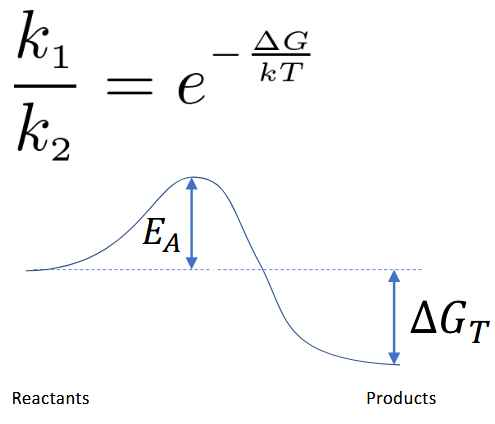
\includegraphics[width=\textwidth]{ArrheniusEquation2}
	\end{subfigure}
	\;
	\begin{subfigure}[t]{0.3\textwidth}
		\caption{The right base versus the wrong base: $\Delta \Delta G$ gives us the ratio of the products, of the right or the wrong type}\label{fig:ArrheniusEquation3}
		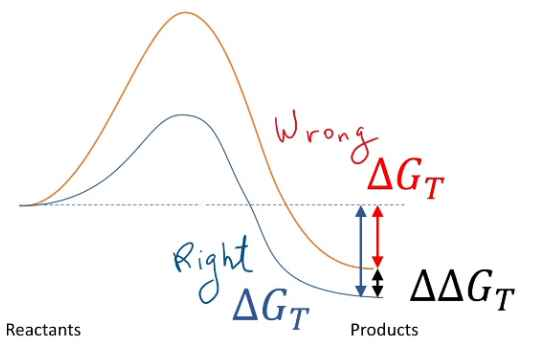
\includegraphics[width=\textwidth]{ArrheniusEquation3}
	\end{subfigure}
\end{figure}


Activation energy is actually often what enzymes affect and also, in this case, what DNA polymerase affects. The reverse reaction will include the same activation energy often--so you will have to go over the same peak. But sometimes, if reactants and products
have different free energy, then there's also $\Delta G$--Figure \ref{fig:ArrheniusEquation2}. So, the activation energy going backwards includes another term,$\Delta G$, and the rate going back could be slower or faster. The ratio between the two gives us then $e^{-\frac{\Delta G}{kT}}$.

And, when we have a case where we are talking about the right base versus the wrong base
we're looking at two different reactions--Figure \ref{fig:ArrheniusEquation3}.
And then, what we're interested in is the $\Delta \Delta G$,
the difference between the two $\Delta G$s, which then gives us the ratio of the products
of the right or the wrong type.

There's also... one can also talk about
the difference in the activation energy,
which is important in DNA polymerase
and we'll talk about later.
But, at first, we'll start with
this $\Delta \Delta G$.
So, does $\Delta \Delta G$,
the difference in binding strength--
difference in the hydrogen bonds--Figure \ref{fig:RightWrong}--does this explain how well DNA bonds? When we start with a certain ratio of right to wrong, then the reaction amplifies the ratio by $e^\frac{\Delta \Delta G}{kT}$


\begin{figure}[H]
	\caption[Start with a certain ratio of right to wrong]{Start with a certain ratio of right to wrong; the reaction amplifies the ratio by $e^\frac{\Delta \Delta G}{kT}$} \label{fig:RightWrong} 
	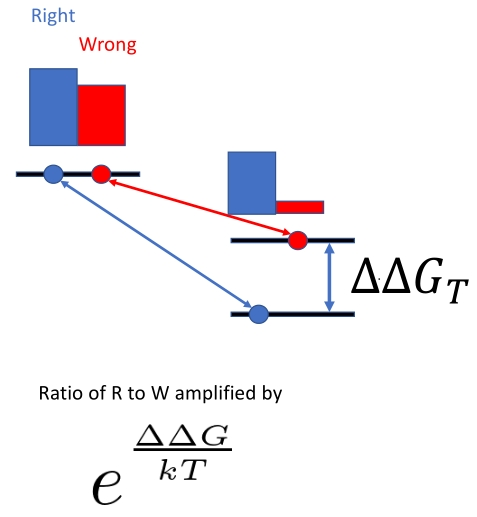
\includegraphics[width=0.9\textwidth]{RightWrong}
\end{figure}

The base pairing energy actually depends on the neighbour bases--Figure \ref{fig:BindingDifference}.
\begin{figure}[H]
	\caption{Difference in Binding Energies for different pairings}
	\begin{subfigure}[t]{0.45\textwidth}
		\caption{The biggest difference between right and wrong is about 2.5 Kcal/mole.} \label{fig:BindingDifference} 
		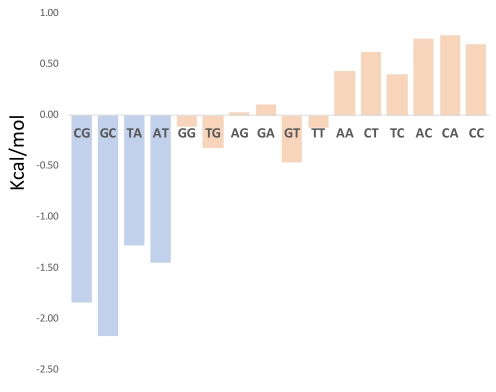
\includegraphics[width=\textwidth]{BindingDifference}
	\end{subfigure}
	\begin{subfigure}[t]{0.45\textwidth}
		\caption{Calculation of $e^\frac{\Delta \Delta G}{kT}$. First term in denominator is Avogadro's number.} \label{fig:BindingDifference1} 
		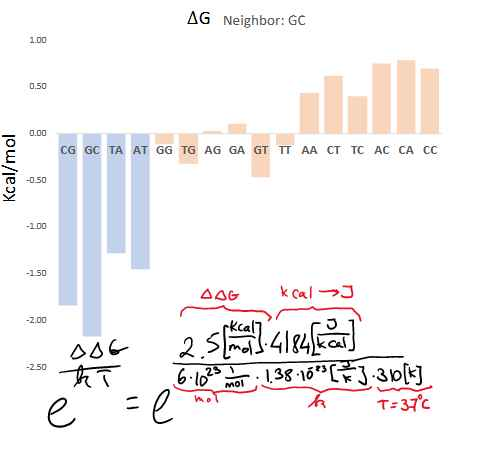
\includegraphics[width=\textwidth]{BindingDifference1}
	\end{subfigure}
	\begin{subfigure}[t]{0.45\textwidth}
		\caption{Next step} \label{fig:BindingDifference2} 
		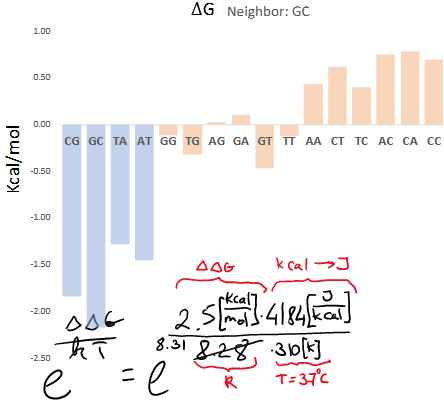
\includegraphics[width=\textwidth]{BindingDifference2}
	\end{subfigure}
	\begin{subfigure}[t]{0.45\textwidth}
		\caption{Result is about 60.} \label{fig:BindingDifference3} 
		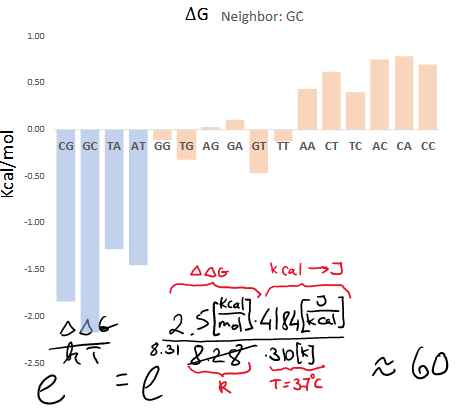
\includegraphics[width=\textwidth]{BindingDifference3}
	\end{subfigure}
\end{figure}

Figure \ref{fig:BindingDifference3} shows that the biggest difference that we would get
just out of the binding energies of base pairs would be a sixty-fold difference,
which is very far from ten to the ten.

How can we get a better effective rate? One proposal that was brought forth is something called ''kinetic proofreading,'' whereby having non-reversible reactions we can actually enhance this ratio. Let's see how it works. We insert an irreversible reaction--Figure \ref{fig:kineticProofreading2}--for an improvement of 3600. Still far from $10^{10}$, but closer.
\begin{figure}[H]
	\caption{Kinetic Proofreading}
	\begin{subfigure}[t]{0.45\textwidth}
		\caption{Reversible reactions--still gives $e^\frac{\Delta \Delta G}{kT}$}\label{fig:kineticProofreading}
		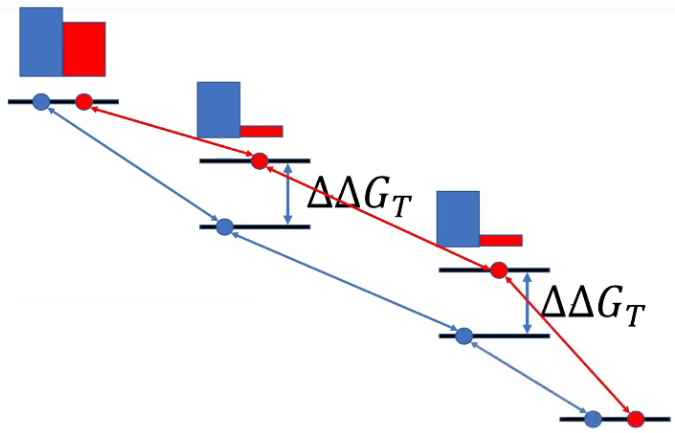
\includegraphics[width=0.8\textwidth]{kineticProofreading}
	\end{subfigure}
	\begin{subfigure}[t]{0.45\textwidth}
		\caption{Insert irreversible reaction--$\big(e^\frac{\Delta \Delta G}{kT}\big)^2$}\label{fig:kineticProofreading2}
		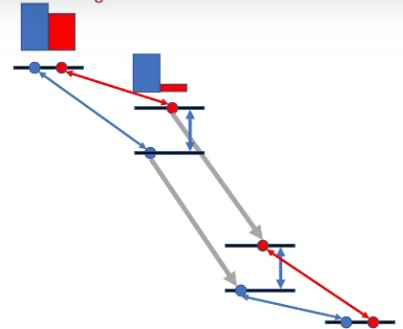
\includegraphics[width=0.8\textwidth]{kineticProofreading2}
	\end{subfigure}
\end{figure}

In the case of DNA polymerase, this is probably not what happens because we don't know of
really an irreversible reaction that uses energy that goes on when we attach another base.
Instead, it seems that, in the case of DNA polymerase, what's important is not really the difference in the free energies, but instead, the shape of the bases.
So, let's look at what DNA polymerase does. 
Figure \ref{fig:WhatDNApolymeraseDoes0} is a schematic representation of DNA polymerase. Usually, it's thought of as something like a hand with fingers and... thumb, and at the bottom you see some DNA polymerases have also the gray exonuclease activity that we'll talk about in a second.

\begin{figure}[H]
	\caption{Schematic representation of DNA polymerase}
	\begin{subfigure}[t]{0.45\textwidth}
		\caption{Usually, it's thought of as something like a hand with fingers and... thumb}\label{fig:WhatDNApolymeraseDoes0}
		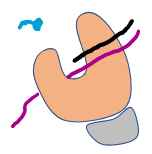
\includegraphics[width=0.8\textwidth]{WhatDNApolymeraseDoes0}
	\end{subfigure}
	\begin{subfigure}[t]{0.45\textwidth}
		\caption{\gls{gls:dNTP} arrives - dNTP is a single base of the DNA that still has the three phosphates attached}\label{fig:WhatDNApolymeraseDoes1}
		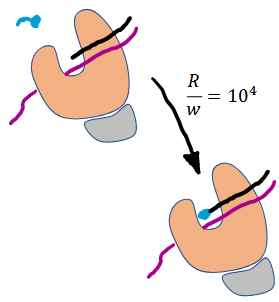
\includegraphics[width=0.8\textwidth]{WhatDNApolymeraseDoes1}
	\end{subfigure}
\end{figure} 


In Figure \ref{fig:WhatDNApolymeraseDoes1}, \gls{gls:dNTP} arrives - dNTP is a single base of the DNA that still has the three phosphates attached.
These three phosphates carry the energy that will be used to bind this base.
Going forward, it seems like the rate of attaching
the right base pair to the wrong one
is about ten to the four. Again, we don't exactly understand
why that is.

Now, once... that base attached,
there's two possibilities
in the case where there is
an exonuclease activity.
We can either go forward
and attach the next base--Figure \ref{fig:WhatDNApolymeraseDoes2}--
or we can a go a bit backward,
move the double-stranded DNA
to a single-stranded DNA,
and move that to the exonuclease part
where the last base pair is removed--Figure \ref{fig:WhatDNApolymeraseDoes}.
And here, the wrong base pair
actually has an advantage
although this happens...
a hundred times more
when the wrong base pair is then
than the right one.
\begin{figure}[H]
	\caption{We can  go forward
		and attach the next base}\label{fig:WhatDNApolymeraseDoes2}
	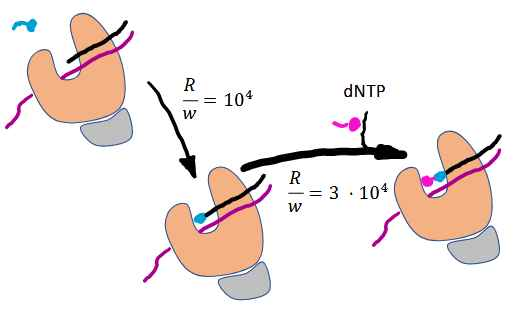
\includegraphics[width=0.8\textwidth]{WhatDNApolymeraseDoes2}
\end{figure} 

\begin{figure}[H]
	\caption[Going backward a bit]{We can a go a bit backward, move the double-stranded DNA to a single-stranded DNA, and move that to the exonuclease part where the last base pair is removed.}\label{fig:WhatDNApolymeraseDoes}
	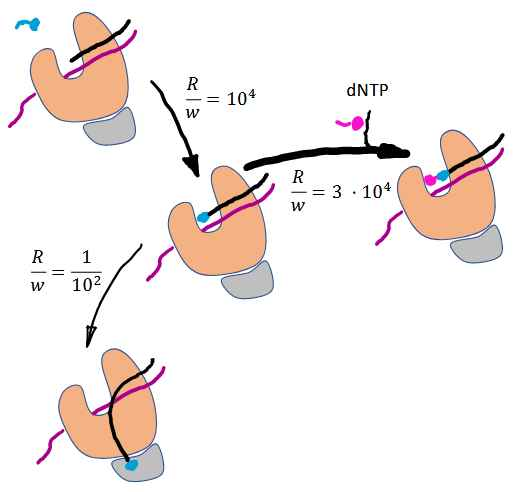
\includegraphics[width=0.8\textwidth]{WhatDNApolymeraseDoes}
\end{figure} 


This together seems to give us a rate
that is close to ten to the ten.
We still don't exactly understand
how all these steps work.
But, it seems what we see is that,
when the base is in the pocket
of the DNA polymerase,
it seems that the shape of the base
and where its every atom is exactly,
determines whether the reaction
will go forward
or go towards the exonuclease activity.
So, the exact shape
of the DNA polymerase -
here I showed  polymerase.
The exact shape is important.
What kind of shapes
will the DNA polymerase encounter?


\subsubsection{Bases encountered by DNA polymerase}
	
\begin{itemize}
	\item Watson Crick pairs (CATG)
	\begin{itemize}
		\item  Binding energy gives ~50 fold enrichment
		\item  Right base at 3-fold disadvantage (compared to the 3 wrong ones)
	\end{itemize}
	\item  ''Valid'' Watson Crick q extra bases (C*,6mA)--so DNA polymerase need to recognize 6 bases, not just 4.
	\begin{itemize}
		\item Additional shapes valid
	\end{itemize}
	\item \gls{gls:NTP} from RNA
	\begin{itemize}
		\item Frequent
		\item Shape recognition--DNA polymerase has a pocket that doesn't alow RNA to get in.
	\end{itemize}
	\item “Nonstandard” bases
	\begin{itemize}
		\item Rare, probably shape recognition
	\end{itemize}
\end{itemize}

\subsubsection{DNA mismatch repair}

A molecule called \emph{MutS} recognizes places where DNA doesn't have the right shape. Mistakes can be made by DNA polymerase, and UV and other external sources can interfere.
\gls{gls:MMR} depends on a molecule, MutS, which looks for places where the DNA doesn't look right, e.g. it has a nick. Because the wrong base was inserted,
it recognized these places.
And then, another molecule, MutL,recognizes -- at least in prokaryotes --a location where
there's a CTAG with 6mA, so a methylated amine--Figure \ref{fig:DNA-MMR}.
When DNA replicates, this methylation is not replicated,
and therefore it's possible to recognize where the old strand is the new strand --
the new strand will not have the A methylated.
And then, at that place... the new strand is nicked,
this whole new strand is removed up to the mismatch,
and then repolymerized by DNA polymerase -
hopefully without an error. So, this is one thing that removes errors
mainly during DNA replication.


\begin{figure}[H]
	\caption{MutL recognizes a location where there's a CTAG with 6mA,}\label{fig:DNA-MMR}
	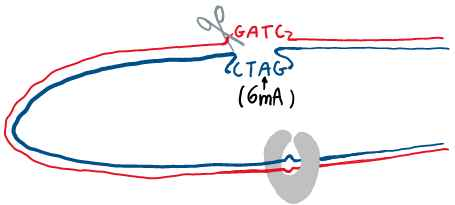
\includegraphics[width=0.8\textwidth]{DNA-MMR}
\end{figure}

Two other mechanisms are direct reversal and base excision.
So, you see here 24 bases that are pretty much specifically recognized for these mechanisms.
\begin{itemize}
	\item Direct reversal --Figure \ref{fig:MMR1} --you reverse exactly the high frequency errors
	that can be introduced by chemistry or UV
	and you revert them to the original base.
    \item Bases excision repair --Figure \ref{fig:MMR2}--you remove again a recognized error, and then that - or a region around it - 	and then DNA polymerase replicates again.
\end{itemize}

\begin{figure}[H]
	\begin{center}
		\caption[Direct Reversal]{Direct Reversal: you reverse exactly the high frequency errors 	that can be introduced by chemistry or UV}\label{fig:MMR1}
		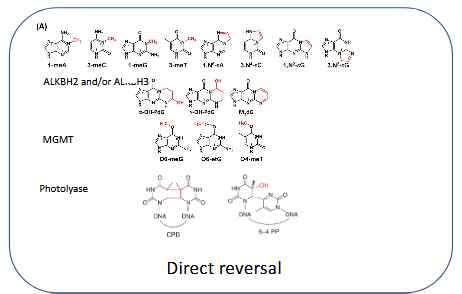
\includegraphics[width=0.8\textwidth]{MMR1}
	\end{center}
\end{figure}

\begin{figure}[H]
	\begin{center}
		\caption{Base excision repair: you remove again a recognized error}\label{fig:MMR2}
		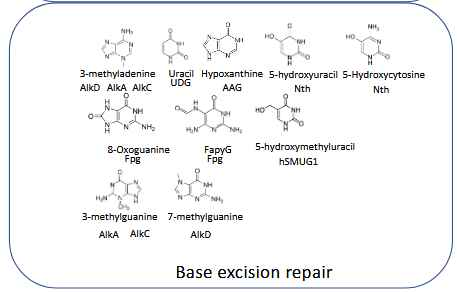
\includegraphics[width=0.8\textwidth]{MMR2}
	\end{center}
\end{figure}

What we see in all these mechanisms is that DNA actually does error corrections through the fact that every bit of information appears twice on one strand and on the other strand.
So, if you know - in the case of MutS - if you know which strand is old and which is new, you can copy the more correct information that doesn't have replication error again.
And, in these cases of reversal or base excision, again, you recognize the error and through that are able to correct.
So, the error correction here uses the fact that DNA is double-stranded.

\subsubsection{Summary}
 It isn’t the bases that make DNA so amazing.
\begin{itemize}
	\item Many bases exist in DNA/RNA
	\begin{itemize}
		\item Damage, modification, insertion
	\end{itemize}
	\item \gls{gls:dNTP} concentration is controlled
	\item DNA polymerase controls	pairing
	\item Large number of specific/general repair enzymes
\end{itemize}

It is only these mechanisms, working together, that give rise to the high fidelity of DNA--\cite{kunkel2004dna}

Sarah added (forum):
\begin{quote}
	The idea of Section \ref{section:DNAasInfo2} is that the thermodynamics alone cannot explain our high fidelity replication, and that our system of replicating DNA uses several compounding mechanisms to generate robust replication. While the first organisms likely lacked this process as the machinery to do this is very sophisticated, it is interesting to consider how early organisms would have survived with less controlled replication. Perhaps indicating that early organisms relied on gene products that had lower specificity?
\end{quote}

\section[Water as a Driving Force for Organization]{Water as a Driving Force for Organization--Sarah Maurer
}

To better understand how living organisms are organized we first need to understand the thermodynamics of aggregation behaviours, and to do this we need to use the equation for thermodynamic free energy (\ref{eq:gibbs}).
\begin{align*}
	\Delta G =& \Delta H - T \Delta S \text{, where}\numberthis \label{eq:gibbs}\\
	G =& \text{ Gibbs Free Energy}\\
	H =& \text{ Enthalpy}\\
	S =& \text{Entropy}
\end{align*}

\begin{table}[H]
	\begin{center}
		\caption{Chemical Energetics}\label{tab:chemical:energetics}
		\begin{tabular}[pos]{|c|c|c|}\hline
			Favourable&Unfavourable/spontaneous&Equilibrium/non-spontaneous\\\hline
			$\Delta G<0$; exergonic&$\Delta G>0$;endergonic&$\Delta G=0$\\\hline
			$\Delta H<0$; exothermic&$\Delta H>0$endothermic&\\\hline
			$\Delta S>0$;less ordered&$\Delta S<0$; more ordered&\\\hline
		\end{tabular}
	\end{center}
\end{table}


\begin{itemize}
	\item  Enthalpy is ”heat” energy, generally stored in bonds
	\begin{itemize}
		\item Breaking bonds takes enthalpy
		\item Making bonds releases enthalpy
	\end{itemize}
	\item Entropy is a measure of the number of occupied states of a system relative to the number of possible	states--Figure \ref{fig:EntropySugar}.
\end{itemize}

\begin{figure}[H]
	\caption{Entropy--$\frac{occupied}{total}$} \label{fig:EntropySugar} 
	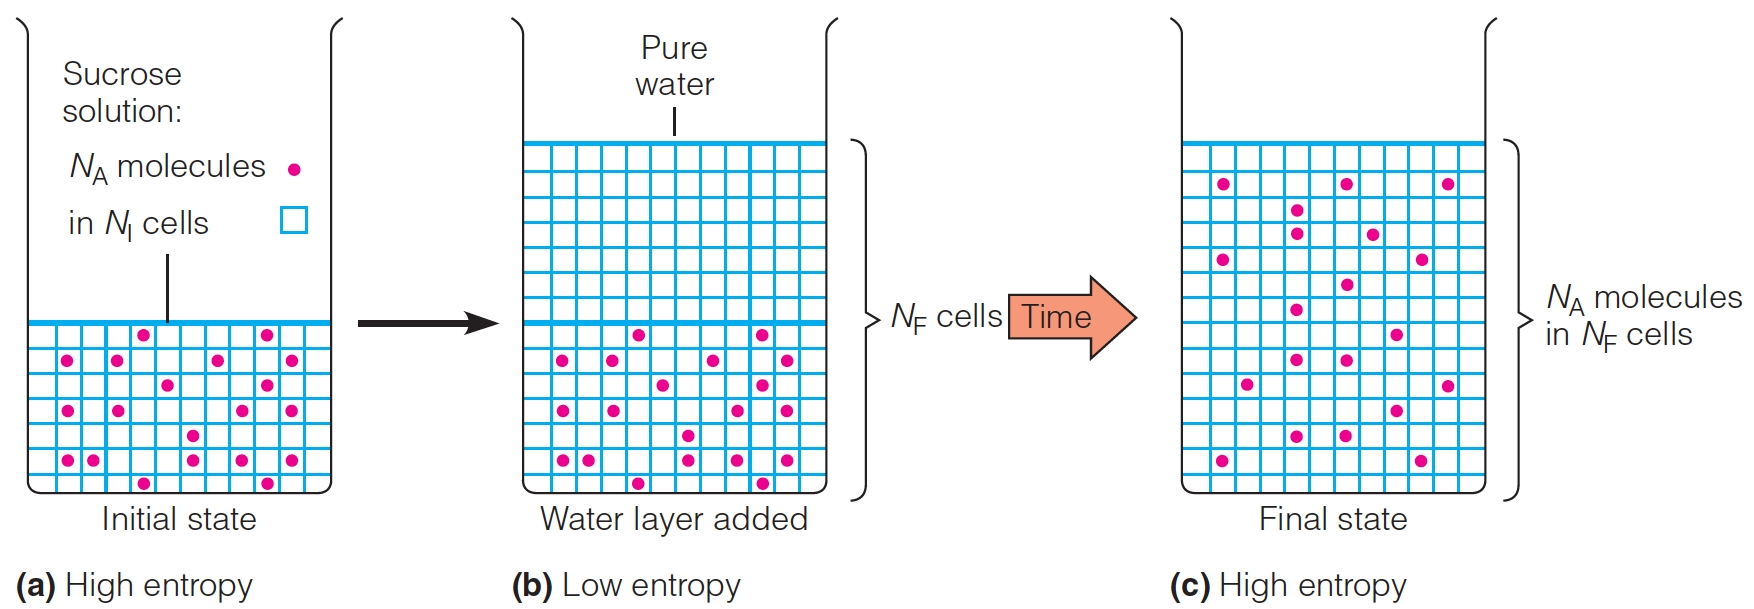
\includegraphics[width=0.9\textwidth]{EntropySugar}
\end{figure}

The enthalpic contribution from water arises from hydrogen bonds, which are not like covalent bonds. They are considered to be intermolecular bonds, so they occur between molecules. They are transient, but they are very strong. They can only form because water is polar. In Figure \ref{fig:EnthalpyHydrogenBonds} the oxygen is negative, and the hydrogen positive. Figure \ref{fig:EnthalpyHydrogenBonds1} shows two water molecules bounds by a hydrogen bond. Very polar bonds can form hydrogen bonds (H-bonds): only F-H, N-H, or O-H, with
N, F or O.

\begin{figure}[H]
	\centering
		\caption{Very polar bonds can form hydrogen bonds} 
	\begin{subfigure}{.5\textwidth}
		\centering
		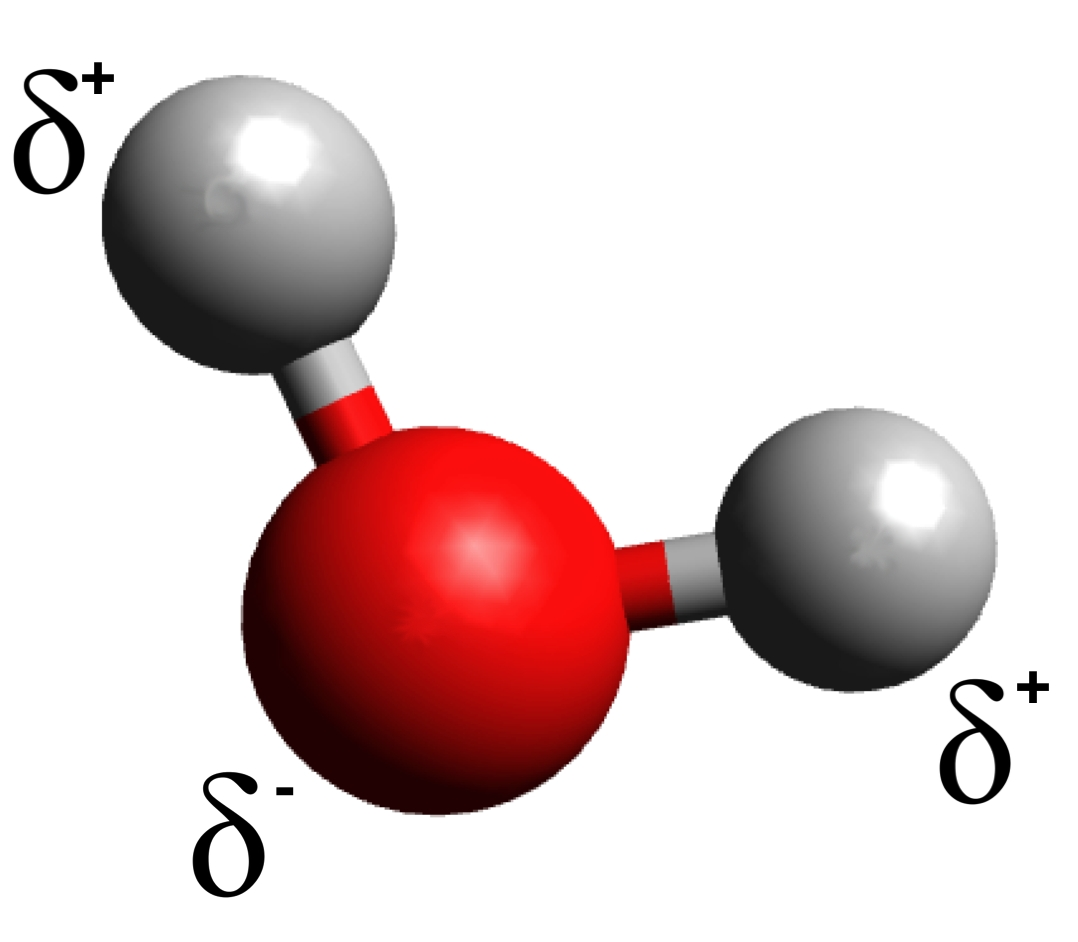
\includegraphics[width=.4\linewidth]{EnthalpyHydrogenBonds}
		\caption{Oxygen accepts electrons from Hydrogen}\label{fig:EnthalpyHydrogenBonds} 
	\end{subfigure}%
	\begin{subfigure}{.5\textwidth}
		\centering
		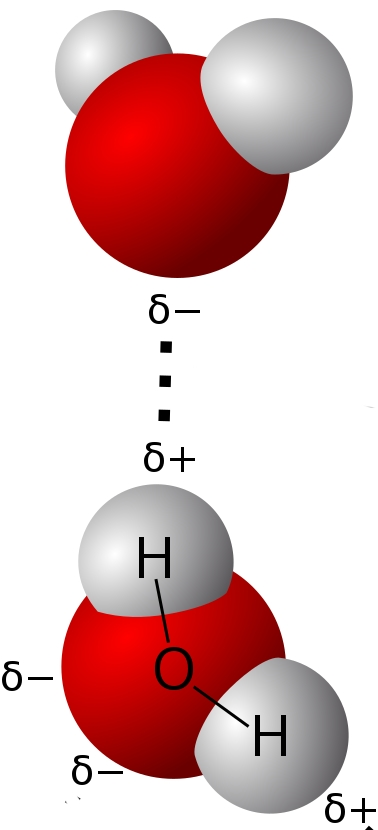
\includegraphics[width=.4\linewidth]{EnthalpyHydrogenBondMore}
		\caption{Positive ends bind to negative}\label{fig:EnthalpyHydrogenBonds1} 
	\end{subfigure}
\end{figure}

\begin{figure}[H]
	\caption{The most important hydrogen bonds for biology} \label{fig:MajorHydrogenBonds} 
	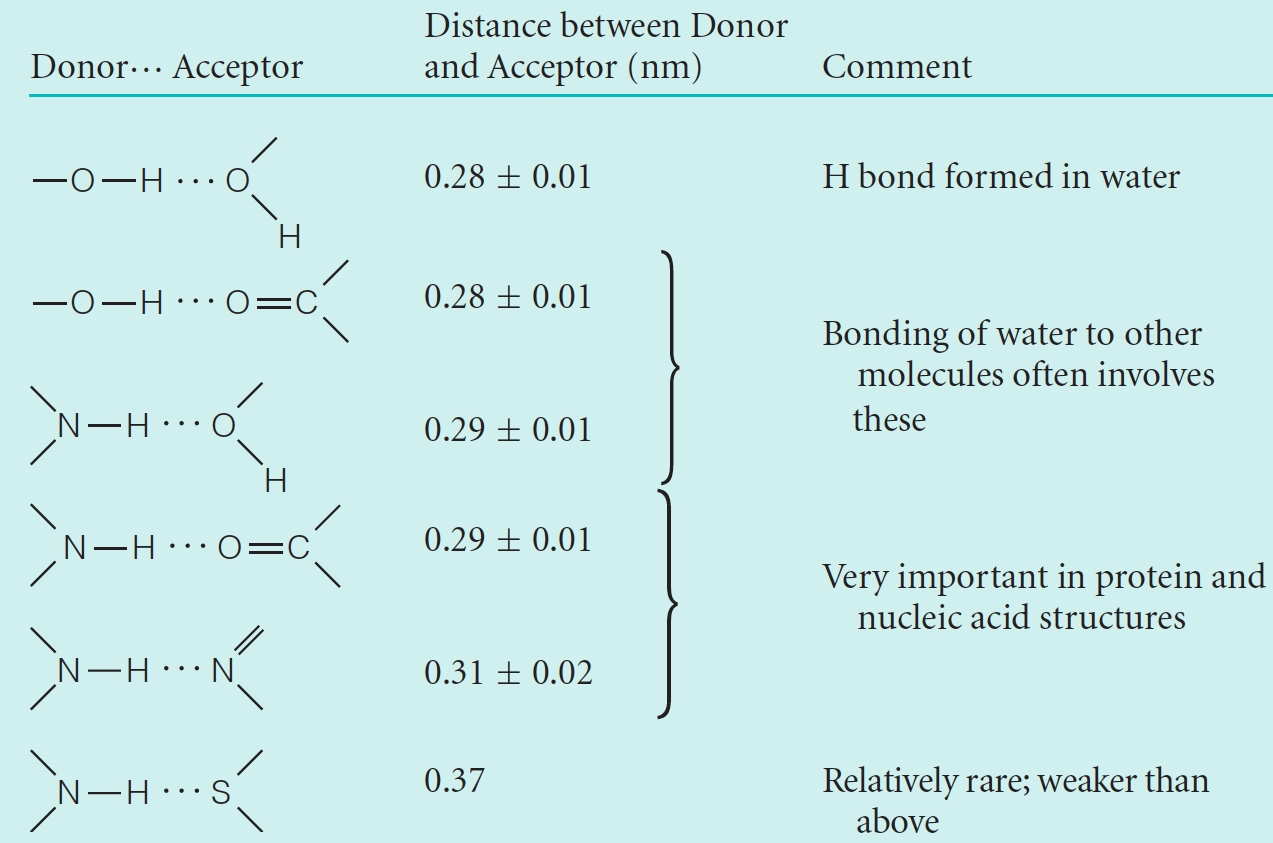
\includegraphics[width=0.9\textwidth]{MajorHydrogenBonds}
\end{figure}

Water has an entropic contribution: it can form many hydrogen bonds	with itself--Figure \ref{fig:Water_H_Bonds}--about 2 or 3 at a time. Molecules change conformation more frequently than once pers second.
\begin{figure}[H]
	\centering
	\caption{Water can form many hydrogen bonds	with itself} \label{fig:Water_H_Bonds} 
	\begin{subfigure}{.66\textwidth}
		\centering
		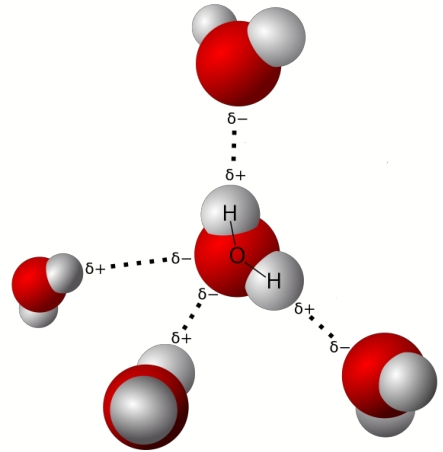
\includegraphics[width=.4\linewidth]{Water_H_Bonds}
		\caption{Water can bind to 2 or 3 others}
		\label{fig:sub1a}
	\end{subfigure}%
	\begin{subfigure}{.33\textwidth}
		\centering
		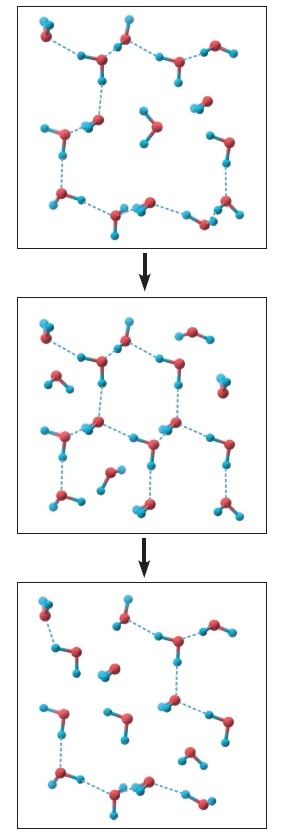
\includegraphics[width=.4\linewidth]{Water_H_Bonds_structure.jpg}
		\caption{Hydrogen bonds constantly change}
		\label{fig:sub2a}
	\end{subfigure}
\end{figure}

\begin{itemize}
	\item Water is good at interacting with polar or charged molecules
	\item ''Like dissolves like''
\end{itemize}

Water is good at interacting with polar or charged molecules. Figure \ref{fig:NonCovalentBonds} shows Sodium Chloride dissolved in water: the Sodium interacts with Oxygen, and Chloride with Hydrogen. This is a little stronger than a water-water interaction, so enthalpy is favoured over the entropic contribution.
\begin{figure}[H]
	\caption{Water is good at interacting with polar or charged
		molecules} \label{fig:NonCovalentBonds} 
	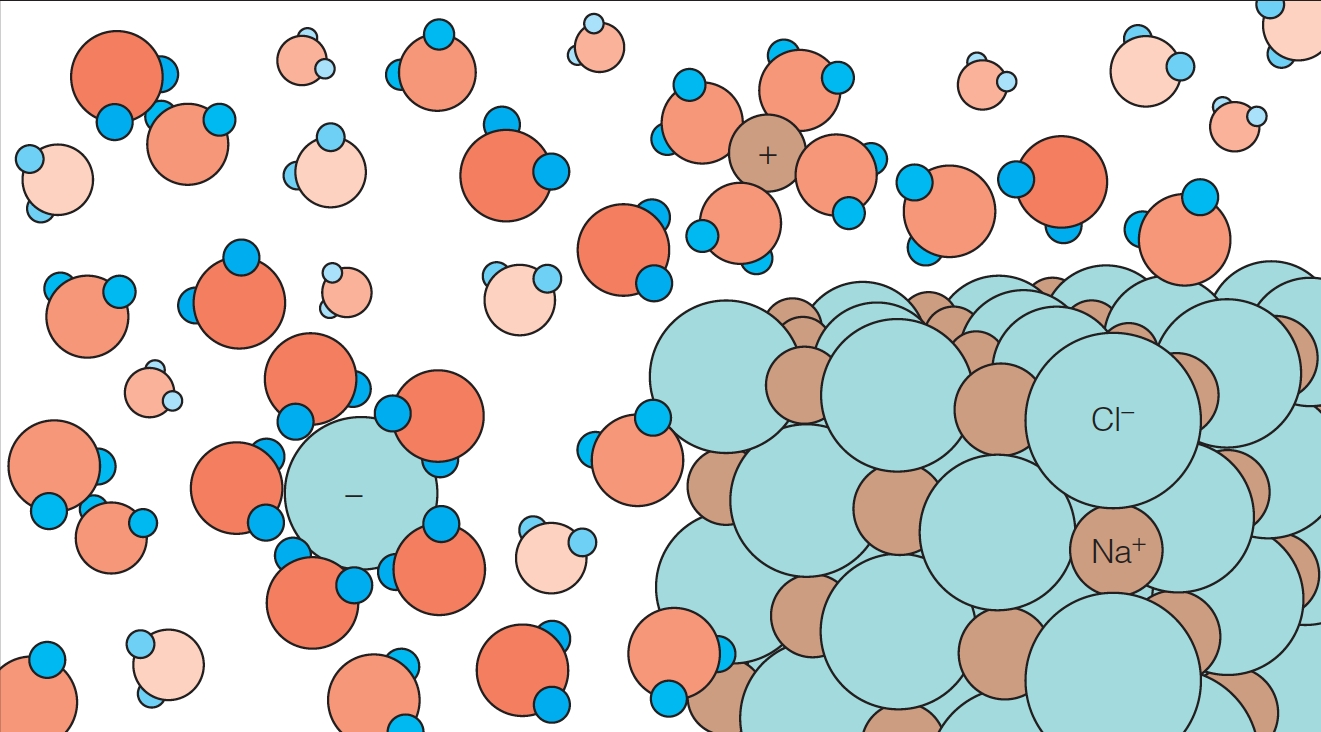
\includegraphics[width=0.9\textwidth]{NonCovalentBonds}
\end{figure}

Oil in Water
\begin{itemize}
	\item Figure \ref{fig:Hexane} depicts the formation of \gls{gls:clathrate} structures – water cannot form hydrogen bonds with oils.
	\item In Figure \ref {fig:clathrate}, Oxygen atoms are shown in red. Hydrogens are shown for one pentagon of oxygens. This is entropically unfavourable, and is known as the hydrophobic effect--Figure \ref{fig:HydrophobicEffect}.
	\item The ordered structure may extend considerably
	further into the surrounding water.
\end{itemize}
\begin{figure}[H]
	\centering
	\caption{Oil in water} \label{fig:Hexane} 
	\begin{subfigure}{.4\textwidth}
		\centering
		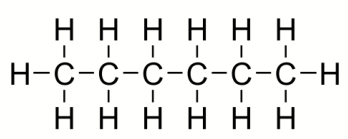
\includegraphics[width=.4\linewidth]{Hexane}
		\caption{Hexane is non-polar}
		\label{fig:hexane}
	\end{subfigure}%
	\begin{subfigure}{.6\textwidth}
		\centering
		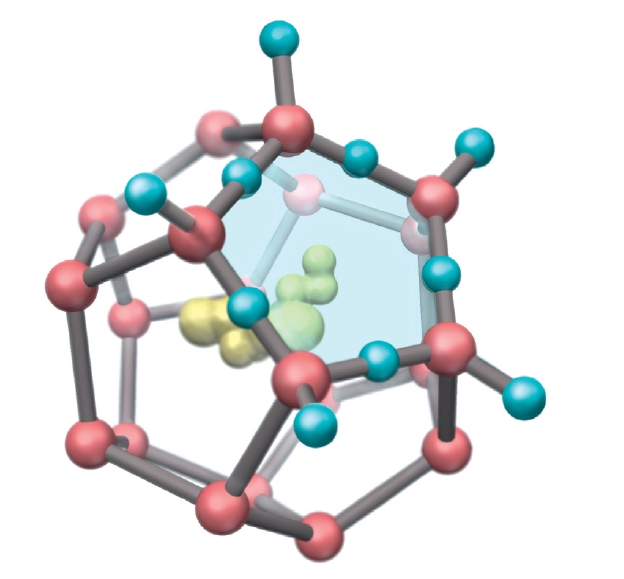
\includegraphics[width=.4\linewidth]{OilInWater.jpg}
		\caption{\Gls{gls:clathrate}: oxygen atoms are shown in red.}
		\label{fig:clathrate}
	\end{subfigure}
\end{figure}

Figure \ref{fig:HydrophobicEffect} depicts the hydrophobic effect: when oil interacts with water, it decreases entropy, which is thermodynamically unfavourable.
The hydrophobic effect leads to the formation of Lipid membranes-- Figure \ref{fig:LiquidMembraneFormation}. 
\begin{figure}[H]
	\caption{Hydrophobic effect} \label{fig:HydrophobicEffect} 
	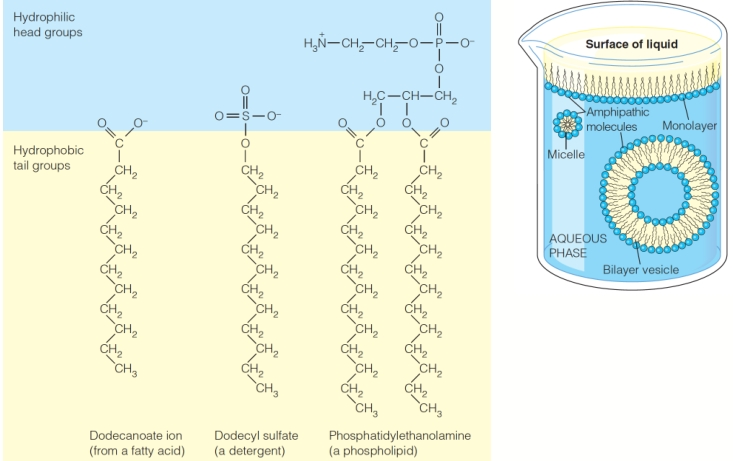
\includegraphics[width=0.9\textwidth]{HydrophobicEffect}
\end{figure}

Lipid membrane formation is depicted in Figure \ref{fig:LiquidMembraneFormation}.

\begin{itemize}
	\item Provides spatial organization within the cell
	\item Allows chemical gradients to generate energy
	\item Individuates populations to allow for Darwinian selection
\end{itemize}

\begin{figure}[H]
	\caption{Lipid membrane formation} \label{fig:LiquidMembraneFormation} 
	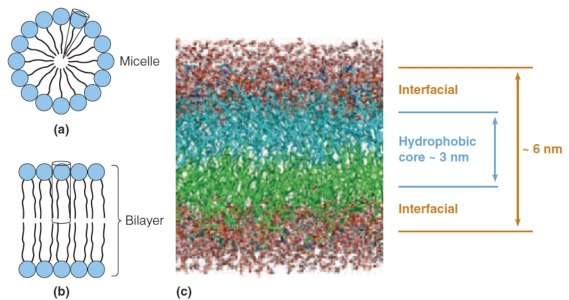
\includegraphics[width=0.9\textwidth]{LiquidMembraneFormation}
\end{figure}

Water also organizes material through Protein Folding, Figure \ref{fig:ProteinFolding} 
\begin{figure}[H]
	\caption{Protein folding} \label{fig:ProteinFolding} 
	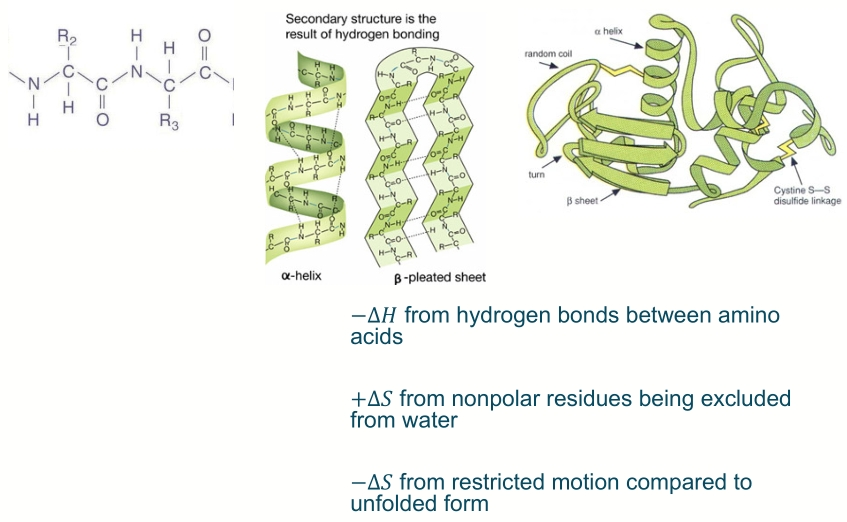
\includegraphics[width=0.9\textwidth]{ProteinFolding}
\end{figure}

 Relevance to origins of life?
\begin{itemize}
	\item Are proteins necessary in first life?
	\item Are membranes necessary in first life?
	\item Is water necessary for life?
\end{itemize}

Even in the RNA world, where RNA can fold and catalyze reaction, folding would be driven by entropy in part. Water is only solvent that has this high entropy. Ammonia can form hydrogen bonds, but they aren't as strong as water. Maybe water is the favoured solvent for life everywhere--\cite{ball2017water}.

\section[Kinetic vs. Thermodynamics – Assembly Constraints]{Kinetic vs. Thermodynamics – Assembly Constraints-- Chris Butch}

\begin{itemize}
	\item \gls{gls:kinetics}  \glsdesc{gls:kinetics}
	\item \gls{gls:thermodynamics} \glsdesc{gls:thermodynamics}
\end{itemize}

A system may be stable in both sense, either, or none--Figure \ref{fig:VisualizingStability}.
\begin{figure}[H]
	\begin{center}
		\caption{VisualizingStability}\label{fig:VisualizingStability}
		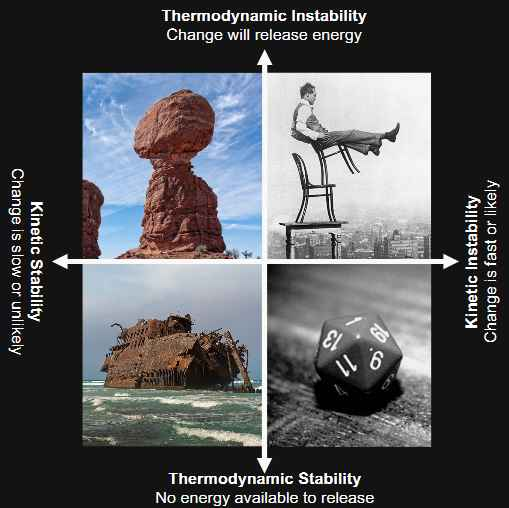
\includegraphics[width=0.6\textwidth]{VisualizingStability}
	\end{center}
\end{figure}

Figure \ref{fig:ApplicationsToChemistry} shows how this applies to chemistry.

\begin{figure}[H]
	\begin{center}
		\caption[Applications to Chemistry]{Applications to Chemistry. In order to exit the left hand state, the system needs to move to a higher energy before falling to low energy state on right.}\label{fig:ApplicationsToChemistry}
		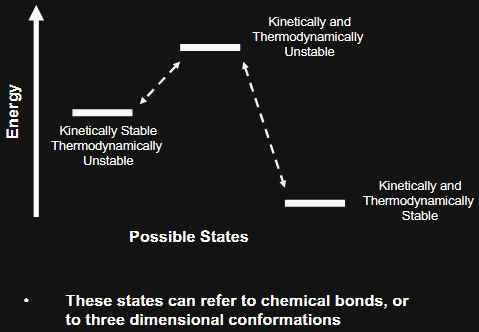
\includegraphics[width=0.6\textwidth]{ApplicationsToChemistry}
	\end{center}
\end{figure}
This is relevant because biomacromolecules are Kinetic Assemblies.
\begin{itemize}
	\item Chemically: Amino Acids and Nucleic Acids are polymerized using energy from polyphosphates
	\item Structurally: Many nucleic acid structures, and most 	protein structures are kinetic minima, but not thermodynamic minima (local minima)
	\begin{itemize}
		\item  Prion diseases involve an autocatalytic transition from the native kinetic state to a (more)stable thermodynamic state.
	\end{itemize}
\end{itemize}

Looking at an example of a prion folding, Figure \ref{fig:prions} shows the PrP protein. Some energy is released by folding into the normal state, which is kinetically stable, but not thermodynamically stable--\cite{dee2016comparing}. Plaques are the lowest energy state. It is difficult to fight disease as this is uphill.

\begin{figure}[H]
	\caption{The PrP protein is stable kinetically , but not thermodynamically.} \label{fig:prions} 
	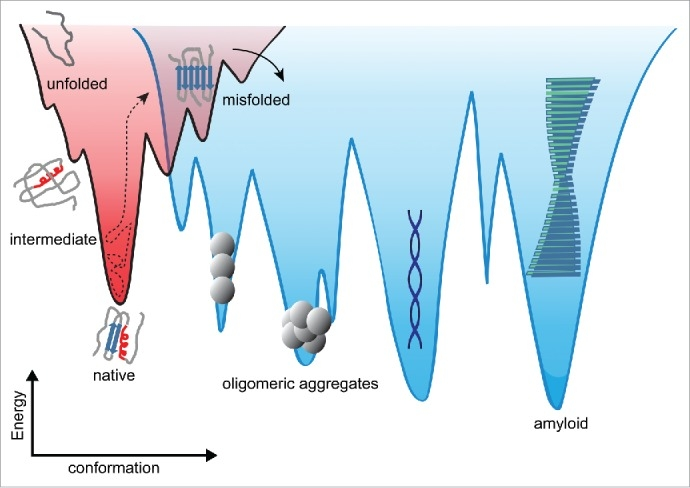
\includegraphics[width=0.9\textwidth]{prions}
\end{figure}

This is also a question for origins of life--Figure \ref {fig:EnergyForOrigin}. How do we drive from a thermodynamic state to a kinetic state?
\begin{figure}[H]
	\caption[Thermal gradients in a pore driving polymerization of nucleic acids]{\cite{mast2013escalation} shows that thermal gradients in a pore, say a pore in a mineral, are capable of driving polymerization of nucleic acids to longer polymers. These polymers are thermodynamically unstable, but kinetically stabilized. We'd like to go further and see folding of polymers and exploration of 3 dimensional spaces. } \label{fig:EnergyForOrigin} 
	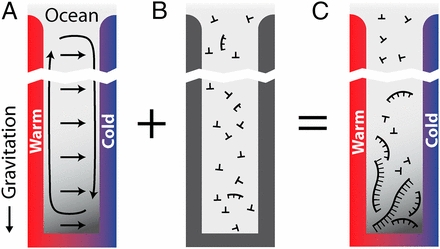
\includegraphics[width=0.9\textwidth]{EnergyForOrigin}
\end{figure}

\textbf{Open Questions}
\begin{itemize}
	\item Do environments exist where biological building blocks such as amino acids are
	thermodynamically favoured, but exploration of their sequence space is kinetically favoured?
	\item How do chemical systems utilize environmental energy to form kinetic assemblies?
\end{itemize}

See \cite{pross2017and,semenov2016autocatalytic,pross2008can,pross2005emergence}.

\section[Chemical Configurations: Proteins and DNA]{Chemical Configurations: Proteins and DNA--Sarah Maurer}

Figure \ref{fig:PrebioticMix} shows the chemicals observed in a Miller-Urey type experiment after \cite{podlech2001origin}. This list isn't what you'd expect to observe if you chopped up a modern cell.
\begin{figure}[H]
	\caption{Prebiotic Mixture from a Miller-Urey type experiment} \label{fig:PrebioticMix} 
	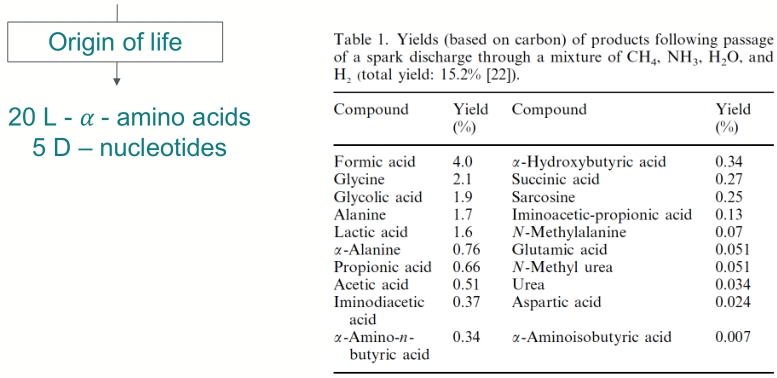
\includegraphics[width=0.9\textwidth]{PrebioticMix}
\end{figure}

\begin{itemize}
	\item How did life select from the list of Figure \ref{fig:PrebioticMix}? E.g. we don't use hydroxybuteric acid.
	\item Life uses L amino acids and D sugars \& nucleotides. How did this come about?
	\item How much of this is prebiotic and how much evolutionary? 
\end{itemize}

\subsection{Chirality}

One major consideration for proteins and nucleic acids is \gls{gls:chirality}--Figure \ref{fig:Chirality1}: all of our amino acids rotate polarized light to the left, and all of our sugars, including those contained in nucleotides, rotate polarized light  to the right. 
 
\begin{figure}[H]
	\caption{Chirality} \label{fig:Chirality1} 
	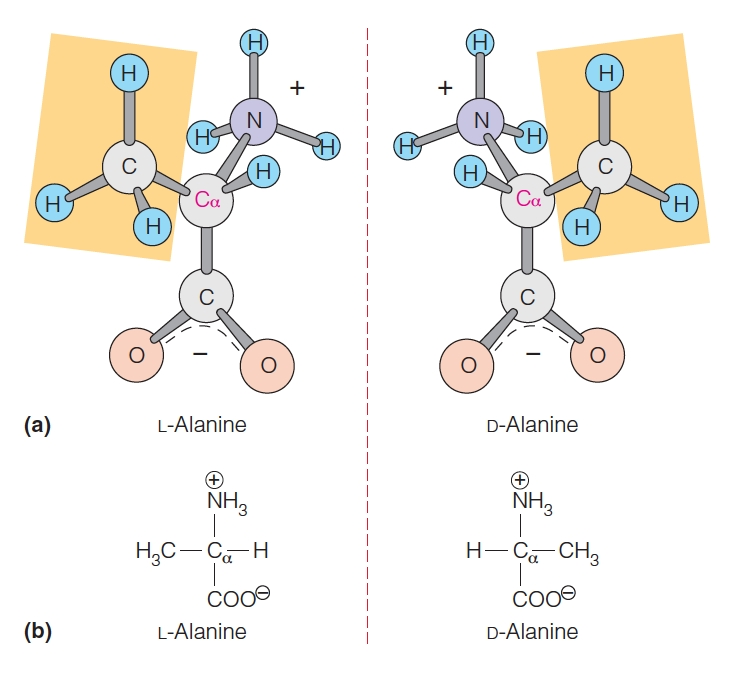
\includegraphics[width=0.9\textwidth]{Chirality1}
\end{figure}

How does chirality arise? Most chemical processes produce equal amounts. At one time it was thought that chirality was a marker for life, but we now know that meteorites are enriched for L--Figure \ref{fig:Chirality2}  \cite{pizzarello2012large}. We call this \gls{gls:enantiomeric-excess}.

\begin{itemize}
	\item L-amino acids – enriched by meteorites----Figure \ref{fig:Chirality2}.
	\item If L-amino acids are polymerized into peptides, and they are reacted with sugars, D-sugars are formed preferentially.
	\item So maybe \gls{gls:chirality} is prebiotic?.
\end{itemize}

\begin{figure}[H]
	\caption{Meteorites are enriched for L} \label{fig:Chirality2} 
	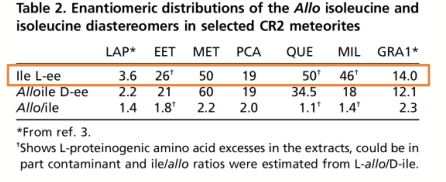
\includegraphics[width=0.9\textwidth]{Chirality2}
\end{figure}


Sarah has added (Forum):
\begin{quotation}
	I know I made it sound like the solution to the chirality of molecules has been found. However this is actually an active area of debate within the community. Many chemical strides have been made in the past 20 year towards making enantiomeric excesses abiotically, and therefore chirality is not specifically thought of as a biological phenomenon. However, to date, there has not been a robust mechanism of generating D-sugars and L-amino acids, although we certainly have seen hints to interstellar generation of excess.
	
	In \cite{soai2019role}, symmetry breaking for a non-biological molecule can be induced by a variety of mechanisms including circularly polarized light and crystal structure.
	
	In \cite{tassinari2019enantioseparation}, the authors use a magnet to crystallize opposite \glspl{gls:enantiomer} of amino acids!
	
	I often refer to chirality as ''the rabbit's hole'' \cite{carroll1898alice} as we have many mechanisms to chase, but it is not obvious if they will get us any closer to understanding origins of life. Or perhaps it is the key to understanding it?
\end{quotation}

\subsection{Amino Acids}

\Gls{gls:chirality} is just one part of the amino acid. There were a lot of molecules in the prebiotic soup that could have become polymers; Table \ref{table:alternatives} shows some alternatives that could have been used.
\begin{table}[H]
	\newlength\mylength
	\setlength\mylength{\dimexpr.33\columnwidth-2\tabcolsep-0.33\arrayrulewidth\relax}
	\caption{Alternatives to the standard Amino Acids}\label{table:alternatives}
	\begin{tabular}{|p{\mylength}| p{\mylength}|p{\mylength}| } \hline
		Biological& Alternatives&Remarks\\ \hline
		Amino acid&	hydroxy acids, thio acids, amino sulfonic- or amino phosphinic acids&Peptide is a very strong bond compared to others. Also amine can hydrogen bond with carboxyl, which is useful for secondary structures. \\ \hline
		Residues at the \gls{gls:alpha:carbon}& $\beta$-, $\gamma$-, or $\delta$-amino acids, or other derivatives&Maybe $\alpha$ more available; also products more stable\\ \hline
		20 exactly& More or less than 20&\\ \hline
		Our specific set of 20 &Other amino acids that were available prebiotically; e.g. why valine and not norvaline?&\\ \hline
	\end{tabular}
\end{table}


Figure \ref{fig:PrebioticAminoAcids} \cite{cleaves2010origin} shows amino acids found in the Murchison meteorite and spark discharges. Some of those which have not been selected for \gls{gls:LAWKI} are more abundant than those that were selected. Why were black ones selected? Maybe they are more stable, or maybe they were incorporated, but later selected against.

\begin{figure}[H]
	\caption{Amino acids found in the Murchison meteorite and spark discharges} \label{fig:PrebioticAminoAcids} 
	\includegraphics[width=0.9\textwidth]{PrebioticAminoAcids}
\end{figure}

Figure \ref{fig:ReducedAlphabet} attempts to reconstruct alphabet at origin; red asterisks are proteins that are not found in prebiotic experiments. The amino acids that have low abundances are the ones that are less likely to be formed. So maybe we started with just a few amino acids and later figured how to synthesize more, and this gave more functionality. 
\begin{figure}[H]
	\caption{Deconstructed Alphabet at time of origin of life} \label{fig:ReducedAlphabet} 
	\includegraphics[width=0.9\textwidth]{ReducedAlphabet}
\end{figure}

More complex amino acids were likely selected based on other criteria(not prebiotic availability), possibly with later adaptation into biochemistry. It is a general rule that the following classes of amino acids are not considered prebiotic.

\begin{itemize}
	\item Sulphur containing
	\item Aromatics
	\item Nitrogen containing
\end{itemize}

We think that chirality and $\alpha$ amino acid structure are prebiotic, but the number of amino acids and their chemical composition could have evolved over time.

\subsection{Nucleic Acid Structure}

Nucleic Acids are a much more complex structure than amino acids: they are not just a backbone and a single side chain. We have bases, sugars, and phosphates--Figure \ref{fig:NucleicAcidStructure}.
\begin{figure}[H]
	\centering
	\caption{DNA/RNA much larger than proteins} \label{fig:NucleicAcidStructure} 
	\begin{subfigure}{.5\textwidth}
		\centering
		\includegraphics[width=.9\linewidth]{NucleicAcidStructure1}
	\end{subfigure}%
	\begin{subfigure}{.5\textwidth}
		\centering
		\includegraphics[width=.9\linewidth]{NucleicAcidStructure2}
	\end{subfigure}
\end{figure}

The phosphate-sugar backbone is much bigger than the amino acid background, and the base is larger than an amino acid. The chemical configuration of a nucleic acid is much more constrained than an amino acid. All nucleic acids are not DNA; there are plenty of naturally occurring nucleic acids--Figure \ref{fig:NaturalxNA}.
\begin{figure}[H]
	\caption{There are natural modified DNAs} \label{fig:NaturalxNA} 
	\includegraphics[width=0.9\textwidth]{NaturalxNA}
\end{figure}

Figure \ref{fig:WhyRibose} depicts the 4 forms of ribose\cite{wei2009permeation}, two \glspl{gls:furan} and two \glspl{gls:pyran}.
\begin{itemize}
	\item Furanoses have $CH_2OH$, needed for polymerization
	\item Need a \gls{gls:beta:anomer} to attach base
	\item Ribose is the only pentose that has plenty of $\beta$ furanose. 
\end{itemize}
\begin{figure}[H]
	\caption[Why Ribose?]{Why Ribose? There are 2 important properties of $\beta$-4-D-Ribofuranose: it has a $CH_2OH$ to attach a phosphate, and it is a \gls{gls:beta:anomer} (OH is up) to attach our base.\label{fig:WhyRibose} }
	\includegraphics[width=0.9\textwidth]{WhyRibose}
\end{figure}

\begin{itemize}
	\item 5-carbon easier to synthesize than 6-, 7-, etc;
	\item shorter sugars don't form ring structure;
	\item so pentoses are cheapest sugar with ring structure.
\end{itemize}

Ribose has an almost unique permeability, so it can enter membrane, pick up phosphate, but cannot get out again! Maybe it was selected for speed?

\begin{figure}[H]
	\caption{These sugars have been tested and can replace Ribose} \label{fig:AlternativeSugars} 
	\includegraphics[width=0.9\textwidth]{AlternativeSugars}
\end{figure}

\begin{figure}[H]
	\caption{Can add a third type of base pair} \label{fig:ExpandGeneticCode} 
	\includegraphics[width=0.9\textwidth]{ExpandGeneticCode}
\end{figure}

Can also modifiy phosphate, as shown in Figure \ref{fig:PhosphateModification}. Oxygen-substitution generates chirality
\begin{itemize}
	\item Boron
	\item Sulfur
	\item Selenium
	\item Hydrogen
\end{itemize}

Improves stability in vivo--useful for gene therapy.

\begin{figure}[H]
	\caption{Phosphate Modification} \label{fig:PhosphateModification} 
	\includegraphics[width=0.9\textwidth]{PhosphateModification}
\end{figure}

Figure \ref{fig:PossibleModifications} shows there are many possible alternatives to DNA/RNA.
\begin{figure}[H]
	\caption{Possible Modifications to DNA} \label{fig:PossibleModifications} 
	\includegraphics[width=0.9\textwidth]{PossibleModifications}
\end{figure}

 More complex amino acids were likely selected based on other criteria (not 
availability), possibly with later adaptation into biochemistry
\begin{itemize}
	\item  Sulfur containing
	\item Aromatics
	\item Nitrogen containing
\end{itemize}
Constraints on origin of amino acids:

\begin{itemize}
	\item  Prebiotic availability
	\item  Metabolic accessibility/compatibility
	\item  Evolutionary history/functional utility
\end{itemize}

How did life choose?

\begin{itemize}
	\item Prebiotic selection:
	\begin{itemize}
		\item 	Availability
		\item Stability of monomers
		\item Stability of polymers
	\end{itemize}
	Biotic selection:
	\begin{itemize}
		\item 	Cost of biosynthesis
		\item Increased functionality
	\end{itemize}
\end{itemize}
Would it choose these twice?

\section{Early Metabolisms}

\subsection[Introduction]{Introduction--Kate Adamala}

All life comes from a starting population of cells--\gls{gls:LUCA}. These cells were the ancestors of all subsequent life, their metabolism shared similarities. We know that the earliest metabolism shared certain features(Figure \ref {fig:LUCA_cell}):
\begin{itemize}
	\item Lipid synthesis--building membranes isolating cells from their surroundings;
	\item Energy: metabolism had to produce \gls{gls:ATP};
	\item \gls{gls:LUCA} was based on proteins made using the current genetic code. We know this because all known organisms on earth share RNA, DNA, and the same genetic code, so this had to be established in \gls{gls:LUCA}. Protein synthesis, and mechanisms such as \gls{gls:tRNA} was a big part of early organisms. 
\end{itemize}

\begin{figure}[H]
	\caption{All life comes from a starting population of cells LUCA} \label{fig:LUCA_cell} 
	\includegraphics[width=0.9\textwidth]{LUCA_cell}
\end{figure}

Figure \ref{fig:LUCA_Environment} depicts a \textit{proposed} reconstruction of the metabolism of \gls{gls:LUCA}. Since early Earth was anoxic, pathways do not use oxygen directly. The Figure is assumed to be near a hydrothermal vent. NB: we don't have any samples of early organisms, so this is a reconstruction based on a study of modern metabolism of all domains of life, and possible environments of early Earth.

The most important element of Figure \ref{fig:LUCA_Environment} are the processes leading to the production of energy. Gradients of ions across the membranes can be used to synthesize \gls{gls:ATP}. Another important mechanism is enzyme \glspl{gls:cofactor}, most notably \gls{gls:SAM}, which is still widely used in modern life, and iron-sulphur clusters. Both of those were likely abundant in earliest metabolisms.

\begin{figure}[H]
	\caption[Proposed main metabolic pathways of LUCA.]{Proposed main metabolic pathways of LUCA. This diagram was created comparing metabolisms, proteins and small molecules of most known modern types of life and finding common shared elements that must have been present in earliest life forms\cite{weiss2016physiology}} \label{fig:LUCA_Environment} 
	\includegraphics[width=0.9\textwidth]{LUCA_Environment}
\end{figure}

All building blocks of life--energy molecules, proteins, nucleic acids, lipids making membranes, are built with carbon.
The process of taking inorganic carbon and converting it into organic carbon building blocks is the key metabolic process of life--Figure \ref{fig:CarbonRules}. Carbon fixation must have been present in \gls{gls:LUCA}, but would have been simpler--fewer and less complex enzymes.
\begin{figure}[H]
	\caption{Carbon fixation} \label{fig:CarbonRules} 
	\includegraphics[width=0.9\textwidth]{CarbonRules}
\end{figure}

Synthesis of Membrane Lipids is another very important metabolic process. Modern cells have two families of Membrane Lipids--Figure \ref{fig:SynthsisMembraneLipids}--the difference is in how a glycerol molecule is derivatized\footnote{\glsdesc{gls:derivatization}} with lipid chains. Bacteria and Eukaryotes share one type, and Archaea have another distinct orientation of the way lipids attach the glycerol. Different enzymes are used to make these two types of lipids. Synthesis of Membrane Lipids was not entirely set at the time of \gls{gls:LUCA}, and was still rapidly evolving. 

\begin{figure}[H]
	\caption[Modern cells have two families of Membrane Lipids]{Modern cells have two families of Membrane Lipids\cite{glansdorff2008last}.} \label{fig:SynthsisMembraneLipids} 
	\includegraphics[width=0.9\textwidth]{SynthsisMembraneLipids}
\end{figure}

We can use this Lipid Synthesis Metabolism Comparison--\ref {fig:LipidSynthesisComparison}--as an example of evolution from earliest ancestors. For some steps there is phylogenetic evidence that homologous mechanisms carried out a particular step or that the enzymes cannot be excluded. Differences between the modern domains of life have to have evolved from the simpler pathways of \gls{gls:LUCA}.
\begin{figure}[H]
	\caption[Lipid Synthesis Metabolism Comparison]{Lipid Synthesis Metabolism Comparison\cite{lombard2012early}} \label{fig:LipidSynthesisComparison} 
	\includegraphics[width=0.9\textwidth]{LipidSynthesisComparison}
\end{figure}

We don't know what the lipid synthesis pathway was in the earliest organisms, but we can be pretty certain that there was a membrane, and we can speculate with a high degree of confidence about the nature of membrane proteins necessary to move nutrients, waste, and signals through those membranes

See also \cite{weiss2016physiology,bar2011survey,fuchs2011alternative}.

\subsection[Energetics]{Energetics--Sarah Maurer}

We look at early metabolisms, and how they evolved into those we see today. 
Figure \ref{fig:ClassificationEnergyGeneration} shows various mechanisms for generating organisms.
\begin{itemize}
	\item \Glspl{gls:chemotroph}--organisms that survive on chemical energy.
	\begin{itemize}
		\item \Glspl{gls:chemoautotroph}--carbon dioxide serves as our carbon source.
		\item \Glspl{gls:chemoheterotroph}--depend on an electron acceptor that is usually oxygen.
	\end{itemize}
	\item \Glspl{gls:phototroph}--organisms that survive on chemical energy.
	\begin{itemize}
		\item \Glspl{gls:photoautotroph}
		\item \Glspl{gls:photoheterotroph}
	\end{itemize}
\end{itemize}

 \Glspl{gls:chemoautotroph} convert $CO_2$ to reduced carbon; this lecture at the evolution of chemoautotrophy. We need to discuss redox reactions, as \glspl{gls:chemoautotroph} need to move electrons around.

\begin{figure}[H]
	\caption{Classification of energy generation in organisms} \label{fig:ClassificationEnergyGeneration} 
	\includegraphics[width=0.9\textwidth]{ClassificationEnergyGeneration}
\end{figure}

We'll think of primordial respiration as a process of electron transfer from sources, such as $Fe^{2+}$ to acceptors--Figure \ref{fig:EvolutionMetabolism}. Free Oxygen would not have been available. Primordial respiration serves as the bases for all later respirations, e.g. the branch for chlorophyll. Later organisms evolve a way of using oxygen as it becomes free.
\begin{figure}[H]
	\begin{center}
		\caption[Evolution of Metabolism]{Evolution of Metabolism (\textit{retinal} should read \textit{retinol})} \label{fig:EvolutionMetabolism} 
		\includegraphics[width=0.9\textwidth]{EvolutionMetabolism}
	\end{center}
\end{figure}

What would the first form of chemoautotrophy have looked like? We think of something like Methanogenesis--Figure \ref{fig:Methanogenesis}, which shows the reduction of carbon in $CO_2$ to $CH_4$. Figure \ref{fig:320px-Methanogenesis_cycle} \cite{wiki:methanogenesis} shows that this is accomplished by attaching $CO_2$ to a larger molecule, and then adding electrons until carbon arrives at its most reduced form. 

\begin{figure}[H]
	\caption[Methanogenesis]{Methanogenesis: $CO_2$ acquires electrons--in red\cite{costa2014metabolic}} \label{fig:Methanogenesis} 
	\includegraphics[width=0.9\textwidth]{Methanogenesis}
\end{figure}

This is a fairly complex process, as shown in Figure \ref{fig:320px-Methanogenesis_cycle}
\begin{figure}[H]
	\caption[Details of reduction of Carbon]{Details of reduction of Carbon\cite{costa2014metabolic}} \label{fig:320px-Methanogenesis_cycle} 
	\includegraphics[width=0.9\textwidth]{320px-Methanogenesis_cycle}
\end{figure}

The mechanism for possible carbon fixation can occur on mineral surfaces. These experiments were specifically done on an iron sulphide surface. We take $CO_2$ and specifically bind it to our mineral surface--the $C\equiv O$ bond in Figure \ref{fig:CarbonFixationMinerals}. This mineral surface is going to act a bit like the methanofuran in methanogenesis, where our carbon dioxide slowly accepts electrons until it turns into the desired products. Here the observed products are formate, methanol, acetate and pyruvate. We don't see lactate.
  
\begin{figure}[H]
	\caption[Carbon Fixation on Minerals]{Carbon Fixation on Minerals (upper path)\cite{varma2018native} } \label{fig:CarbonFixationMinerals} 
	\includegraphics[width=0.9\textwidth]{CarbonFixationMinerals}
\end{figure}

This is exciting because we use pyruvate to generate ATP.
If there is a simple, mineral bound, mechanism for methanogenisis, we think we have a good chance of recreating the actual primordial metabolism for chemoautotrophy in our labs today.

How do electrons move when we have reduced carbon? Figure \ref{fig:ModernRedox} shows how this works today: a citric acid cycle, which generates FADH and $FADH_2$; we have fatty acid oxidation and glycolysis, protein degradation, etc. This all feeds electrons into our electron transport chain, which generates a proton gradient, eventually producing ATP. So essentially we want to take electrons and make a proton gradient that can be used later to drive ATP synthesis.

\begin{figure}[H]
	\caption{Modern Redox Chemistry: the Citric Acid Cycle} \label{fig:ModernRedox} 
	\includegraphics[width=0.9\textwidth]{ModernRedox}
\end{figure}

So what might our early redox chemistries have looked like? Figure \ref{fig:PrimordialRedox} depicts one proposal. At a hydrothermal group we could have a very fine layer of minerals that could act as a porous membrane or electron transfer membrane between alkaline hydrothermal vent and an acidic ocean. So there is already a proton gradient with a pH of 6. Electrons are transferred to $FeS$ and then onto $CO^2$. 



\begin{figure}[H]
	\caption[Primordial Redox Chemistry]{One possible mechanism for primordial Redox Chemistry--\cite{sojo2016origin}. } \label{fig:PrimordialRedox} 
	\includegraphics[width=0.9\textwidth]{PrimordialRedox}
\end{figure}

Other mechanisms have been proposed:
\begin{align*}
H_2 \rightarrow & 2H^+ + 2 e^- \text{, then electrons pushed to $CO^2$ to make formaldehyde}\\
FeS + H_2 S \rightarrow &Fe S_2 +H2\\
4H_2 +CO2 \rightarrow & CH_4 + 2H_2 O\\
4H_2 + 2HCO^-_3 + sH^+\rightarrow & CH_3OO^- + 2H_2O\\
H_2 + Fd_{ox} \rightarrow & Fd^{2-}_{red} + 2H^+ 
\end{align*}

\begin{figure}[H]
	\caption{Evolution of Redox Reactions} \label{fig:PrimordialRedox2} 
	\includegraphics[width=0.9\textwidth]{PrimordialRedox2}
\end{figure}

\section[Energy Harvesting]{Energy Harvesting--Shawn McGlynn}

Why do chemical reactions occur?

\begin{itemize}
	\item Chemical reactions occur when concentrations change to accommodate energy differences between molecules--Figure \ref{fig:EnergyHarvest}.
	
	\item Equilibrium occurs at some mixture of A and B when energy is equalized. The final concentrations are achieved at equilibrium.
	
\end{itemize}

\begin{figure}[H]
	\begin{center}
		\caption[What energy is being harvested?]{Chemical reactions occur when concentrations change to accommodate energy differences between molecules}\label{fig:EnergyHarvest}
		\includegraphics[width=0.5\textwidth]{EnergyHarvest}
	\end{center}
\end{figure}

\begin{itemize}

	\item At constant temperature and 	pressure, we refer 	to the energy that is available to do work as \gls{gls:gibbs-free}, after J. Willard Gibbs--Figure \ref{fig:ReactionEnergies}.
	
	\item $\Delta G$ is the change in energy as a reaction tends towards equilibrium--Figure \ref{fig:ReactionEnergies1}.
	
	\item Biology chains reactions, so one reaction that is energetically unfavourable ( $\Delta G > 0$) may become favourable if coupled to another with  $\Delta G < 0$--Figure \ref{fig:CoupledReactions}. 
\end{itemize}

\begin{figure}[H]
	\begin{subfigure}[t]{0.3\textwidth}
		\caption{Reaction Energies}\label{fig:ReactionEnergies}
		\includegraphics[width=0.9\textwidth]{ReactionEnergies}
	\end{subfigure}
	\begin{subfigure}[t]{0.3\textwidth}
		\caption{Energy quantitatively describes reaction favourability and direction}\label{fig:ReactionEnergies1}
		\includegraphics[width=0.9\textwidth]{ReactionEnergies1}
	\end{subfigure}
	\begin{subfigure}[t]{0.3\textwidth}
		\caption{Biology chains reactions}\label{fig:CoupledReactions}
		\includegraphics[width=0.9\textwidth]{CoupledReactions}
	\end{subfigure}
\end{figure}

Figure \ref{fig:EnergyHarvesting1} examines how this could work in a biological system.

\begin{figure}[H]
	\caption{The cellular membrane 	can separate charge} \label{fig:EnergyHarvesting1} 
	\includegraphics[width=0.9\textwidth]{EnergyHarvesting1}
\end{figure}

Let's explore how this might work. 

\begin{itemize}
	\item In Figure \ref{fig:ChemioOsmosis0} we have zoomed in on the membrane of a bacterium. There is some reaction that is favourable.

	\item Biology couples one type of reaction to another-- Figure \ref{fig:ChemioOsmosis1}--where the reaction is being coupled with moving a proton from the inside of the cell to the outside.

	\item Repeating, we move many protons from the inside to the outside--Figure \ref{fig:ChemioOsmosis2}.
	
	\item In this way we build a a charge imbalance--Figure \ref{fig:ChemioOsmosis3}--which can be used to force some other reaction. We can think of this as using the energy released by $X\rightarrow Y$ to drive $A\rightarrow B$.

\end{itemize}

\begin{figure}[H]
	\caption{How do cells use their membranes to couple chemical reactions?}\label{fig:ChemioOsmosis}
	\begin{subfigure}[t]{0.45\textwidth}
		\caption{Membrane of a bacterium. There is some reaction that is favourable.}\label{fig:ChemioOsmosis0}
		\includegraphics[width=0.9\textwidth]{ChemioOsmosis0}
	\end{subfigure}
	\begin{subfigure}[t]{0.45\textwidth}
		\caption{Chemical reactions can be coupled together: in this case the reaction is being coupled with moving a proton from the inside of the cell to the outside}\label{fig:ChemioOsmosis1}
		\includegraphics[width=0.9\textwidth]{ChemioOsmosis1}
	\end{subfigure}
	\begin{subfigure}[t]{0.45\textwidth}
		\caption{Repeating, we move many protons from the inside to the outside}\label{fig:ChemioOsmosis2}
		\includegraphics[width=0.9\textwidth]{ChemioOsmosis2}
	\end{subfigure}
	\begin{subfigure}[t]{0.45\textwidth}
		\caption{ChemioOsmosis1}\label{fig:ChemioOsmosis3}
		\includegraphics[width=0.9\textwidth]{ChemioOsmosis3}
	\end{subfigure}
\end{figure}

Let's look at some specific examples of how biology actually does this. Figure \ref{fig:ProtonPump1} illustrates one mechanism, where light provides the energy. Other mechanisms, such as Figures \ref{fig:ProtonPump2} and \ref{fig:ProtonPump3} don't involve light: the energy is obtained from the electron-donor.

\begin{figure}[H]
	\caption{Mechanisms for pumping electrons}
	\begin{subfigure}[t]{0.3\textwidth}
		\caption{Bacteriorhodopsin: light provides the energy}\label{fig:ProtonPump1}
		\includegraphics[width=\textwidth]{ProtonPump1}
	\end{subfigure}
	\begin{subfigure}[t]{0.3\textwidth}
		\caption{The movement of electrons can be coupled to the movement of protons: here is an Electrogenic pump where charge goes onto $A$.}\label{fig:ProtonPump2}
		\includegraphics[width=\textwidth]{ProtonPump2}
	\end{subfigure}
	\begin{subfigure}[t]{0.3\textwidth}
		\caption{It’s possible to put charge into the membrane}\label{fig:ProtonPump3}
		\includegraphics[width=\textwidth]{ProtonPump3}
	\end{subfigure}
\end{figure}


Another Variety of charge separating that we see in biology is called the Redox loop. This doesn't involve a pump, but instead it involves the movement of electrons in and protons out. Figure \ref{fig:RedoxLoop1} involves two different proteins, and have two different proteins is key for this mechanism to occur.
Where electrons and protons are picked up and let go makes a big difference. A very good way to build up a charge imbalance if Proton Consumption inside the cell--Figure \ref{fig:ProtonConsumption}.
\begin{figure}[H]
	\caption{The Redox Loop}
	\begin{subfigure}[t]{0.45\textwidth}
		\caption{The protein that strips electrons from $X$ passes them to $A$, which circulates and passes them on to $Y$. The nett result is the electrons move in, and the protons out.}\label{fig:RedoxLoop1}
		\includegraphics[width=\textwidth]{RedoxLoop1}
	\end{subfigure}
	\begin{subfigure}[t]{0.45\textwidth}
		\caption{Proton consumption offers a way of building up a charge difference}\label{fig:ProtonConsumption}
		\includegraphics[width=\textwidth]{ProtonConsumption}
	\end{subfigure}
	\begin{subfigure}[t]{0.3\textwidth}
		\caption{Where electrons and protons are picked up and let go makes a big difference.}\label{fig:RedoxLoop2}
		\includegraphics[width=\textwidth]{RedoxLoop2}
	\end{subfigure}
	\begin{subfigure}[t]{0.3\textwidth}
		\caption{Where electrons and protons are picked up and let go makes a big difference.}\label{fig:RedoxLoop3}
		\includegraphics[width=\textwidth]{RedoxLoop3}
	\end{subfigure}
	\begin{subfigure}[t]{0.3\textwidth}
		\caption{Where electrons and protons are picked up and let go makes a big difference.}\label{fig:RedoxLoop4}
		\includegraphics[width=\textwidth]{RedoxLoop4}
	\end{subfigure}
\end{figure}

There are many mechanisms to move charge across the membrane--Figure \ref{fig:ManyMechanisms}. Today we have only talked about a few of them.
It's important to remember how modular these are, and often in biology you'll find pieces of one pump mixed with another pump next to a redox loop. Biology has explored this space for billions of years.


\begin{figure}[H]
	\caption{Many mechanisms to move charge across the membrane}\label{fig:ManyMechanisms}
	\includegraphics[width=0.9\textwidth]{ManyMechanisms}
\end{figure}

After all this pumping occurs, in general we can imagine doing work with the charge across the membrane. The most famous example is ATPase--Figure \ref{fig:ATPase}--another example of coupling one not-quite-favourable reaction to another.

\begin{figure}[H]
	\caption{ATPase: the charge difference across the membrane is coupled to ATP formation. }\label{fig:ATPase}
	\includegraphics[width=0.8\textwidth]{ATPase}
\end{figure}

\begin{itemize}
	\item Were any of these processes important for the origin of life?
	\begin{itemize}
		\item Many of them are very complicated.
		\item The clouds in Figures \ref{fig:ChemioOsmosis} through \ref{fig:ATPase} are very complicated multimeric protein machines.
		\item They are very complicated, and it difficult for researchers to understand them. \begin{itemize}
			\item Maybe they were too complicated for the origin of life.
			\item Or maybe the origin of life required the development of these machines.
		\end{itemize}
	\end{itemize}
	\item Were the first life forms cellular?
	\begin{itemize}
		\item Could they have been a-cellular?
		\item If not all these talk about bioenergetics becomes difficult to imagine.
		\item Maybe there were other ways of coupling one chemical to another.
	\end{itemize}
	\item If cellular, what type of membrane would they have had?
	\item How would they have pumped?
\end{itemize}

See also \cite{alberts2013essential,simon2008organisation,weizmann2020eQuilibrator}

\section{Systematics and Limits of Metabolic Rates--Chris Kempes}

All present day life is encapsulated: bacteria are simple cells; eukaryotes have organelles, within cells, within multicellular organisms.
\begin{itemize}
	\item Which aspects of extant life are general and 	which are arbitrary?
	\item What can be said about encapsulation in general?
\end{itemize}

How do nutrients cross cell boundary to drive metabolism--Figure \ref{fig:Encapsulation1}?
\begin{figure}[H]
	\caption{Metabolism in Cells} \label{fig:Encapsulation1} 
	\includegraphics[width=0.9\textwidth]{Encapsulation1}
\end{figure}

We model this by the diffusion equation:
\begin{align*}
\frac{\partial C}{\partial t} =& \frac{D}{r^2} \frac{\partial}{\partial r}\big(r^2 \frac{\partial C}{\partial R} \big) \\
\frac{\partial C}{\partial t} =& 0 \text{, in the steady state.}\\
 \frac{D}{r^2} \frac{\partial}{\partial r}\big(r^2 \frac{\partial C}{\partial R} \big) =& 0 \text{, in the steady state.}\\
 r^2 \frac{\partial C}{\partial R} =& A {, say}\\
 C =& B - \frac{A}{r}\\
 \text{assume}& \\
 C =& C_{\infty}\text{, when $r=\infty$, then}\\
 C =& C_{\infty} - \frac{A}{r}
 \text{Further, assume}&\\
 C =& 0\text{, when $r=a$, then we have}\\
 C =& c_{\infty}\big(1 - \frac{a}{r}\big) 
\end{align*}

\begin{align*}
J \triangleq& -D \frac{\partial C}{\partial R}\text{, definition of Flux}\\
=& D C_\infty \frac{a}{r^2}\\
4 \pi a^2 J =& 4 \pi D a C_{\infty} \text{, total flux}
\end{align*}

This gives a limit on the reaction rate of reactions within cells, and shows its dependence on the cell size. 
% end of text 

% glossary
\printglossaries

% bibliography goes here
 
\bibliographystyle{unsrt}
\addcontentsline{toc}{section}{Bibliography}
\bibliography{origins,wikipedia}

\end{document}
